\documentclass[conference]{IEEEtran}
\IEEEoverridecommandlockouts

\usepackage{cite}
\usepackage{amsmath,amssymb,amsfonts}
\usepackage{graphicx}
\usepackage{booktabs}
\usepackage{tabularx}
\usepackage{hyperref}
\usepackage{algorithm}
\usepackage{algorithmic}
\usepackage{textcomp}
\usepackage{xcolor}
\usepackage{multirow}
\usepackage{listings}
\usepackage{tikz}
\usepackage{pifont}
\usepackage{caption}
\newcommand{\cmark}{\ding{51}}
\newcommand{\xmark}{\ding{55}}
\usetikzlibrary{arrows.meta,positioning,fit,shapes.misc,calc}
\usepackage{xcolor}
\lstset{
    basicstyle=\ttfamily\footnotesize,
    keywordstyle=\color{blue},
    commentstyle=\color{gray},
    stringstyle=\color{red},
    breaklines=true,
    columns=fullflexible,
}

\lstdefinelanguage{Solidity}{
    keywords={pragma, solidity, contract, function, public, external, view, returns, mapping, struct, event, emit, if, for, while, require, assert, revert, address, bytes32, uint, uint8, uint64, uint256, string, bool, calldata, memory, storage, indexed, indexed, onlyAdmin, onlyPolicyAdmin},
    keywordstyle=\color{teal}\bfseries,
    ndkeywords={function, return, mapping, struct, event, emit, require},
    ndkeywordstyle=\color{brown},
    identifierstyle=\color{black},
    sensitive=false,
    comment=[l]{//},
    morecomment=[s]{/*}{*/},
    commentstyle=\color{gray}\ttfamily,
    stringstyle=\color{red},
    morestring=[b]",
    morestring=[b]'
}


\def\BibTeX{{\rm B\kern-.05em{\sc i\kern-.025em b}\kern-.08em
    T\kern-.1667em\lower.7ex\hbox{E}\kern-.125emX}}

\begin{document}

\title{Action-Aware ABAC for Heterogeneous Insurance Evidence: Architecture, Evaluation and Results}


\author{\IEEEauthorblockN{Anthony Uchenna Eneh $^{1}$, Love Allen Chijioke Ahakonye $^{2}$, Jae Min Lee $^{1}$, Dong-Seong Kim $^{1}$ $^{\ast}$} 
\IEEEauthorblockA{$^{1}$ IT-Convergence Engineering, \textit{Kumoh National Institute of Technology}, Gumi, South Korea \\
$^{\ast}$ NSLab Co. Ltd., Gumi, South Korea,
\textit{Kumoh National Institute of Technology}, Gumi, South Korea}
\IEEEauthorblockA{$^{2}$ ICT Convergence Research Center, 
\textit{Kumoh National of Technology}, Gumi, South Korea}
{(anthony, loveahakonye, dskim, ljmpaul)}@kumoh.ac.kr}
\maketitle

\begin{abstract}
Auto-insurance platforms rely on cloud infrastructure to store and process diverse
evidence assets including first notice of loss (FNOL) reports, medical documents,
telematics logs, photographs, and high-resolution accident videos. Although recent
blockchain approaches provide tamper resistance and partial access control, they lack
a unified, enforceable model capable of governing heterogeneous resources, supporting
action-level permissions, and binding authorization decisions to off-chain storage.
This paper introduces \textbf{ClaimGuard}, a PureChain-backed, verifiable,
attribute-based access control (ABAC) architecture designed for multi-stakeholder
auto-insurance evidence workflows. ClaimGuard evaluates subject, object, action, and
contextual attributes on-chain and issues short-lived capability tokens to securely
mediate access to cloud/IPFS evidence while ensuring auditability, revocation, and
resilience against honest-but-curious cloud providers. A comprehensive evaluation
compares ClaimGuard with a baseline cloud-only role-based access control (RBAC)
model across varying load, policy-update frequency, policy churn under scale, and
adversarial scenarios, both on local networks (Hardhat) and public testnets (Sepolia).
Results show that ClaimGuard introduces modest latency overhead on local networks 
(60.9\,ms P50 vs.\ 1.9\,ms for pure RBAC) while significantly improving authorization 
correctness, policy integrity, and cross-organizational trust. Policy evaluation latency 
remains stable (2--3\,ms median) from 11 to 1{,}000 active rules, and revocation propagates 
within 1.1\,ms. Public testnet evaluation validates feasibility on real blockchain 
infrastructure. The system fills a key gap identified in the literature by providing 
the first resource-agnostic, action-aware, enforceable access control framework tailored 
to the operational requirements of modern auto-insurance evidence management.
\end{abstract}

\section{Introduction}

Auto-insurance platforms increasingly rely on large volumes of heterogeneous
digital evidence, including first notice of loss (FNOL) reports, medical and
repair documents, telematics logs, photographs, sensor traces, and
high-resolution accident videos. These assets are accessed throughout the claim
lifecycle—submission, assessment, investigation, fraud analysis, legal escalation,
and regulatory auditing—by diverse stakeholders such as insurers, reinsurers,
loss adjusters, police, courts, repair vendors, and regulators. Cloud-based
systems provide the scalability required for handling such evidence; however,
they also require full trust in the cloud operator and expose sensitive data to
insider threats, misconfiguration, and inconsistent enforcement of access
policies. Recent surveys of blockchain applications in insurance and intelligent
transportation systems consistently identify access control as one of the least
resolved and most operationally critical challenges in these ecosystems
\cite{pournader2020blockchaininsurance, xu2021survey, yli2020blockchain}.

Existing approaches fall broadly into two categories: cryptography-driven
evidence sharing and blockchain-enhanced workflow integrity. Prior works
introducing CP-ABE or proxy re-encryption for insurance data
\cite{sun2020insurance, wang2020secure, liu2021auto, brousmiche2018hybrid}
provide confidentiality for specific types of evidence but tightly couple
authorization to encryption policies and do not generalize to heterogeneous
evidence or multi-actor workflows. Meanwhile, blockchain-based insurance systems
typically employ role-based access control (RBAC) or smart-contract modifiers to
protect claim functions \cite{raikwar2018insurance, tekale2023claims,
thukral2023vehicle, hombalimath2024vehicleclaim, raghav2024optimizing,
alwis2022decentralized}, but these mechanisms enforce only coarse authorization
(e.g., “insurer”, “police”, “court”) and fail to capture fine-grained,
action-level or context-aware permissions across diverse evidence types.

Broader vehicular and intelligent transportation literature provides additional
context. Solutions such as \cite{syed2020vehicle, brousmiche2018digitizing,
singh2020vcare, singh2019ubi} emphasize data provenance, IoT integration, and
secure sharing, but do not provide mechanisms for expressively controlling
read, append, update, delete, adjudication, or disclosure permissions over
multi-format evidence stored off-chain. Related work in healthcare data sharing
\cite{sun2020emr, rana2022healthcare, liang2017mhealth, theodouli2018healthcare}
demonstrates strong patient-centric authorization but assumes constrained
stakeholder sets and cannot satisfy the complex, multi-organization
requirements of auto-insurance workflows.

Collectively, these limitations reveal a persistent gap: no existing system
provides an end-to-end, verifiable, tamper-resistant access-control architecture
that is resource-agnostic, action-aware, context-sensitive, and enforceable over
off-chain cloud storage. Critical capabilities—fine-grained authorization,
purpose constraints, time windows, revocation, temporary access (e.g., for
police or courts), and protection from honest-but-curious cloud providers—remain
unaddressed. Moreover, the literature lacks quantitative evaluation comparing
blockchain-backed access control with baseline cloud-only RBAC under realistic
workloads and adversarial conditions.

To address these gaps, this paper introduces \textbf{ClaimGuard}, a PureChain-
backed attribute-based access control (ABAC) architecture for multi-stakeholder
auto-insurance evidence workflows. ClaimGuard evaluates subject, object, action,
and contextual attributes on-chain and mediates access to cloud/IPFS resources
via a policy-aware enforcement gateway that issues short-lived capability
tokens. By anchoring policy evaluation in tamper-resistant smart contracts and
decoupling authorization from data encryption, ClaimGuard provides auditability,
revocation, and protection against over-privileged cloud operators.

We further develop a simulation environment to compare ClaimGuard with a
cloud-only RBAC baseline, evaluating latency, throughput, policy-update
overhead, authorization correctness, and resilience to unauthorized access.
Results show that ClaimGuard introduces modest overhead while significantly
improving policy integrity, enforceability, and cross-organizational trust.

Section~II reviews related work. Section~III formalizes access-control
requirements for auto-insurance evidence. Section~IV presents the ClaimGuard
architecture. Section~V discusses the security posture and threat mitigations.
Section~VI describes the experimental methodology. Section~VII presents results
and analysis. Section~VIII concludes the paper.

\section{Related Work and Novelty}

\subsection{Blockchain-Based Access Control in Insurance}
Sun \emph{et al.}~\cite{sun2020insurance} propose a blockchain--IPFS insurance data storage scheme that integrates ciphertext-policy attribute-based encryption (CP-ABE) to provide fine-grained access control. Their system focuses primarily on cryptographic enforcement and outsourced encryption via fog nodes. However, the approach is tightly coupled to CP-ABE encryption policies and offers no architectural mechanism for binding on-chain policies to off-chain object stores or for modeling multi-stakeholder auto-insurance workflows involving police, courts, repair vendors, and reinsurers.

Liu \emph{et al.}~\cite{liu2021auto} design a blockchain-based auto-insurance data sharing scheme using proxy re-encryption to allow authorized users to decrypt shared claim data. The work addresses secure data sharing but does not define a generalized access control model across heterogeneous evidence types such as FNOL forms, medical records, telematics logs, videos, and PDF documents. Moreover, it does not specify an action-aware permission model or enforcement gateway that mediates access to cloud or IPFS resources.

Raikwar \emph{et al.}~\cite{raikwar2018insurance} introduce a blockchain-centered framework for generic insurance processes, with smart contracts managing state transitions between clients and agents. Although confidentiality and restricted access to client data are discussed, access control remains role-oriented and process-specific; evidence-level authorization, revocation, purpose restriction, and multi-actor collaboration are not modeled.

Tekale and Rahul~\cite{tekale2023claims} apply blockchain and smart contracts to claims settlement workflows, introducing role-based access control (RBAC) to regulate claim state transitions. While this contributes to process integrity, RBAC over state transitions does not generalize to fine-grained ABAC over diverse auto-insurance evidence assets, nor does it provide an enforceable architecture for cloud storage access.

\subsection{Access Control in Healthcare and DLT}
A substantial body of work explores blockchain-enabled access control for electronic medical records (EMR) and healthcare data sharing~\cite{liang2017mhealth,theodouli2018healthcare,sun2020emr,rana2022healthcare}. These systems often employ ABE or smart-contract-based authorization to govern data access among patients, doctors, health insurers, and pharmacies. Although conceptually related, these works address healthcare contexts and rely on domain-specific assumptions such as patient-centric ownership, decryptable EMR bundles, and limited stakeholder sets. They do not extend to auto-insurance evidence pipelines involving dynamic evidence creation, partial disclosure, legal time windows, or multi-party investigative processes.

\subsection{Gaps in Existing Literature}
Across insurance- and healthcare-oriented blockchain systems, the following limitations persist:
\begin{itemize}
    \item Access control mechanisms are either cryptographic (CP-ABE, proxy re-encryption) or role-based, with no general-purpose attribute-based model governing evidence objects and actions.
    \item Evidence assets are typically treated as a single type (e.g., images, EMR records), whereas real auto-insurance workflows involve heterogeneous documents, media, sensor data, and derived reports.
    \item Prior architectures lack a policy enforcement gateway that binds on-chain access decisions to off-chain cloud/IPFS objects using short-lived capabilities.
    \item Revocation, time-bounded access, purpose-of-use restrictions, cross-insurer collaboration, and legal-access workflows are inconsistently addressed or entirely absent.
    \item No work offers a system-level, simulation-based comparison between blockchain-backed access control and traditional cloud-only RBAC in terms of latency, throughput, scalability, and access correctness.
\end{itemize}

\subsection{Discussion of Comparative Analysis}

\begin{table*}[t]
\centering
\caption{Comparison of Related Blockchain-Based Access Control Systems}
% Reduce padding to fit within margins while keeping normal font size
\setlength{\tabcolsep}{3pt}
\begin{tabularx}{\textwidth}{l l X X X c X X}
	\toprule
	\textbf{Work} & \textbf{Domain} & \textbf{Evidence Types} & \textbf{Access Model} & \textbf{Action-Aware} & \textbf{On-Chain Policies} & \textbf{Off-Chain Enforcement} & \textbf{Evaluation Style} \\
\midrule
Sun et al. (2020) \cite{sun2020insurance} & Insurance data & Images / records & CP-ABE & No & Partial (ABE policies) & No & Cryptographic analysis \\
Liu et al. (2021) \cite{liu2021auto} & Auto insurance & Claim documents & Proxy Re-Enc. & No & Limited & No & Security + cost analysis \\
Raikwar et al. (2018) \cite{raikwar2018insurance} & Generic insurance & Process states & RBAC (workflow) & Limited & Yes & No & Qualitative \\
Tekale \& Rahul (2023) \cite{tekale2023claims} & Claim settlement & Claim states & RBAC (roles) & Yes (states only) & Yes & No & Conceptual \\
Sun et al. (2020) EMR \cite{sun2020emr} & Healthcare & EMR bundles & ABE & No & No (ABE only) & No & Scenario-driven \\
Rana et al. (2022) \cite{rana2022healthcare} & Healthcare & EMR, identity & Smart-contract ABAC & Partial & Yes & No & Conceptual \\
Liang et al. (2017) \cite{liang2017mhealth} & Mobile healthcare & Patient data & Permission protocol & No & Yes & No & Conceptual \\
Theodouli et al. (2018) \cite{theodouli2018healthcare} & Healthcare sharing & Records & Smart contracts & No & Yes & No & Architectural \\
\midrule
	\textbf{This Work} & \textbf{Auto-insurance evidence} & \textbf{FNOL, PDFs, images, telematics, videos} & \textbf{PureChain ABAC} & \textbf{Yes (CRUD, append, adjudicate)} & \textbf{Yes (Verifiable contract rules)} & \textbf{Yes (Gateway + capabilities)} & \textbf{Simulation vs RBAC baseline} \\
\bottomrule
\end{tabularx}
\label{tab:comparison}
\end{table*}

Table~\ref{tab:comparison} summarizes the distinguishing characteristics of 
prior blockchain-based access control systems across insurance, healthcare, and 
generic data-sharing domains. Existing insurance-oriented schemes either rely 
on cryptographic primitives such as CP-ABE~\cite{sun2020insurance} or proxy 
re-encryption~\cite{liu2021auto}, or they implement fixed RBAC rules embedded 
within smart contracts for workflow transitions~\cite{raikwar2018insurance,
tekale2023claims}. These approaches offer selective confidentiality or 
process-level authorization but do not generalize to the diverse evidence 
types and fine-grained action semantics present in auto-insurance workflows.

Healthcare-focused systems~\cite{sun2020emr,rana2022healthcare,
liang2017mhealth,theodouli2018healthcare} demonstrate the utility of 
blockchain-backed permissions, yet they operate under patient-centric data 
models and typically enforce access at the level of decryptable record bundles. 
None provide a unified attribute-based policy model for controlling heterogeneous 
evidence assets nor an architectural mechanism to enforce blockchain decisions 
over cloud or IPFS object storage.

As the table indicates, no prior work simultaneously provides: 
(i) resource-agnostic and action-aware ABAC policies, 
(ii) verifiable on-chain policy evaluation, 
(iii) off-chain enforcement through a policy-aware gateway, and 
(iv) a system-level performance comparison against baseline cloud-only RBAC. 
These gaps collectively motivate the architecture and evaluation presented in 
this paper.


\subsection{Novelty of This Work}
This paper contributes a unified, resource-agnostic, action-aware access control architecture for auto-insurance evidence workflows. To the best of our knowledge, it is the first to:
\begin{enumerate}
    \item Model the \textbf{full multi-stakeholder auto-insurance evidence lifecycle} using an attribute-based access control (ABAC) framework covering subjects, objects, actions, and contextual constraints such as legal windows and investigative purpose.
    \item Implement these policies in \textbf{PureChain smart contracts}, decoupling policy verification from data encryption and enabling tamper-resistant authorization across insurers, police, courts, repair shops, and regulators.
    \item Introduce a \textbf{policy enforcement gateway} that binds on-chain decisions to off-chain cloud/IPFS resources via short-lived capability tokens, ensuring enforceability against an honest-but-curious cloud provider.
    \item Support \textbf{revocation, partial disclosure, action-level permissions}, and workflow-driven context attributes absent in prior insurance access control schemes.
    \item Provide a \textbf{simulation-based evaluation} comparing PureChain-backed ABAC with cloud-only RBAC under varied load, policy-update frequency, and adversarial conditions.
\end{enumerate}

Together, these contributions position the proposed architecture as the first end-to-end, verifiable, and enforceable access control system tailored for the operational realities of auto-insurance evidence management.


\section{Problem Definition and Requirements}

Auto-insurance workflows involve the continuous generation, storage, exchange,
and verification of heterogeneous evidence assets across multiple organizations.
This section formalizes the problem context motivating a verifiable and
action-aware access control framework, identifies key actors and threat
assumptions, and derives explicit functional and security requirements for an
architecture capable of governing evidence access over cloud-based storage
using blockchain-backed policies.

\subsection{System Context}

The auto-insurance evidence pipeline consists of multiple stages: 
(1) incident occurrence and First Notice of Loss (FNOL), 
(2) evidence collection (images, videos, telematics logs, medical documentation, repair estimates), 
(3) claim creation and assessment, 
(4) investigation or dispute resolution (e.g., fraud analysis, police or court access), 
and (5) settlement and regulatory auditing. 
Evidence assets are stored predominantly in cloud object stores or IPFS 
repositories due to their size and format diversity, while insurance consortia
increasingly employ permissioned or consortium blockchains to maintain 
tamper-resistant audit trails, policy state, and transaction logs.  
Access to these assets must be authorized according to business logic, legal 
mandates, and privacy constraints, yet enforced over off-chain storage that is 
not inherently governed by blockchain semantics.

\subsection{Stakeholders and Roles}

The system involves a broad set of stakeholders with differing access rights and
contextual constraints:
\begin{itemize}
    \item \textbf{Policyholder / Vehicle Owner:} Submits FNOL and provides 
    evidence (images, videos, telematics data, statements).
    \item \textbf{Primary Insurer:} Assesses claims, validates supporting 
    evidence, performs fraud checks, and communicates with other stakeholders.
    \item \textbf{Reinsurer / Secondary Insurers:} Require partial evidence for 
    proportional coverage or multi-party claims.
    \item \textbf{Repair Workshops and Assessors:} Need controlled access to 
    vehicle condition evidence, repair estimates, and inspection reports.
    \item \textbf{Law Enforcement (Police):} Require incident evidence for 
    investigations, often under time-limited and legally mandated access.
    \item \textbf{Judicial Bodies (Courts):} May require temporary read access 
    or controlled disclosure during litigation.
    \item \textbf{Regulators and Auditors:} Require immutable logs of access 
    events and selective evidence access for compliance.
    \item \textbf{Cloud Providers (Untrusted):} Store raw evidence assets but 
    must not gain access to plaintext or unmediated retrieval privileges.
\end{itemize}

The diversity of stakeholders, evidence types, and permissible actions
necessitates a fine-grained and auditable access-control model.

\subsection{Threat Model}

We assume the following realistic threat environment:
\begin{itemize}
    \item \textbf{Honest-but-curious cloud provider:} Controls the storage layer
    but must not be able to view, tamper with, or enumerate evidence without a
    capability token or explicit authorization.
    \item \textbf{Compromised organizational insider:} An authorized stakeholder 
    (e.g., adjuster or workshop staff) may attempt to overreach permissions by 
    accessing evidence belonging to unrelated claims.
    \item \textbf{External attacker:} Attempts to intercept capability tokens, 
    steal credentials, replay requests, or directly query cloud storage.
    \item \textbf{Malicious stakeholder:} A party may try to manipulate access 
    rights, backdate evaluations, or circumvent revocation.
    \item \textbf{Network adversary:} May observe or tamper with 
    communication between API gateways, blockchain nodes, or cloud endpoints.
\end{itemize}

The adversary cannot break standard cryptographic primitives but may exploit 
design flaws, misconfigurations, temporal inconsistencies, or lack of 
revocation semantics.

\subsection{Evidence Assets and Actions}

Auto-insurance evidence is heterogeneous and includes:
\begin{itemize}
    \item \textbf{Structured documents:} FNOL, medical reports, invoices,
    estimates, communication logs, adjuster notes.
    \item \textbf{Unstructured media:} Photos, video footage, audio recordings.
    \item \textbf{Sensor data:} Telematics, speed/acceleration logs, GPS traces.
    \item \textbf{Derived artifacts:} Fraud indicators, AI-generated summaries,
    expert assessments, compressed clips.
\end{itemize}

Different stakeholders must perform different actions over these assets:
\begin{itemize}
    \item \textbf{Read:} Download, preview, analyze, or review evidence.
    \item \textbf{Write/Append:} Add new evidence files, attach statements, or
    update claim information.
    \item \textbf{Update/Modify:} Correct FNOL, upload revised repair estimates,
    or append new medical updates.
    \item \textbf{Delete (rare, controlled):} Remove erroneously uploaded
    evidence; requires strong permissions and audit.
    \item \textbf{Adjudicate:} Mark evidence as admissible, confirmed, disputed,
    or legally sealed.
    \item \textbf{Disclose:} Temporarily grant access to police, courts, or
    third-party investigators.
\end{itemize}

A robust access control model must be capable of evaluating permissions over this 
full action space.

\subsection{Representative Scenarios}

Several core scenarios highlight the necessity of a general-purpose, verifiable 
ABAC approach:

\subsubsection{Scenario 1 - Claim Assessment}
A policyholder uploads videos and photos. The primary insurer and authorized 
adjusters require read and append privileges for additional documentation, while 
repair workshops require partial read access only for vehicle-condition evidence.

\subsubsection{Scenario 2 - Legal Investigation}
Police obtain temporary read-only access to specific media files related to an 
incident. Courts may require additional disclosure with strict expiration times,
and revocation must be enforced immediately after the legal window closes.

\subsubsection{Scenario 3 - Multi-Insurer Coordination}
Reinsurers require controlled access to FNOL, telematics summaries, and repair 
estimates but not medical data or unrelated claim materials.

\subsubsection{Scenario 4 - Fraud Detection}
Investigators need access to historical claim patterns and aggregated evidence,
but only for cases explicitly assigned to them, with strong auditability.

These scenarios motivate a need for verifiable, context-aware, and 
fine-grained access control spanning heterogeneous assets.

\subsection{Design Constraints}

Any practical access control architecture for auto-insurance evidence must
address several constraints:
\begin{itemize}
    \item \textbf{C1: Off-chain storage dominance.} Evidence objects are too 
    large or too diverse for on-chain storage, necessitating secure off-chain 
    access enforcement.
    \item \textbf{C2: Multi-organizational governance.} No single entity can be 
    trusted to maintain unilaterally modifiable access rules.
    \item \textbf{C3: Auditability and non-repudiation.} All policy updates and 
    access decisions must be verifiable and immutable.
    \item \textbf{C4: Context dependence.} Access often depends on time, 
    jurisdiction, investigation stage, or explicit legal mandates.
    \item \textbf{C5: Revocation responsiveness.} Access granted for temporary 
    purposes (e.g., police access) must be revocable with immediate effect.
    \item \textbf{C6: Minimal cloud trust.} Cloud providers must not unilaterally 
    infer, retrieve, or leak evidence.
\end{itemize}

\subsection{Access Control Requirements}

Based on the above analysis, the system must satisfy the following requirements:

\begin{itemize}
    \item \textbf{R1: Fine-Grained, Resource-Agnostic ABAC.} Policies must apply 
    uniformly to all evidence types (documents, media, sensor logs, derived 
    objects) without media-specific assumptions.
    \item \textbf{R2: Action-Aware Authorization.} Authorization must incorporate 
    explicit actions (read, append, update, delete, adjudicate, disclose) rather 
    than only access/no-access.
    \item \textbf{R3: Multi-Attribute Context Evaluation.} Policies must evaluate 
    subject attributes (role, affiliation, jurisdiction), object attributes (type, 
    case ID, sensitivity), and contextual constraints (time windows, legal 
    purpose, workflow stage).
    \item \textbf{R4: Verifiable Policy Governance.} Access rules and updates must 
    be stored on a tamper-resistant blockchain, ensuring transparent, 
    cross-organizational governance.
    \item \textbf{R5: Enforceable Off-Chain Access Binding.} Decisions made on 
    the blockchain must translate into enforceable access over cloud/IPFS storage 
    via short-lived capability tokens or equivalent mechanisms.
    \item \textbf{R6: Revocation and Temporal Control.} The system must support 
    immediate revocation and time-bounded access to satisfy legal and 
    investigative requirements.
    \item \textbf{R7: Auditability and Non-Repudiation.} All access events must be 
    logged and attributable to specific stakeholders.
    \item \textbf{R8: Least Privilege and Delegation.} Stakeholders may only 
    access the minimal evidence required for their task; temporary delegation 
    must be possible with full traceability.
    \item \textbf{R9: Resilience to Cloud and Insider Threats.} Cloud providers 
    and insiders must not obtain unauthorized access even if they control the 
    storage layer or possess internal credentials.
\end{itemize}

\subsection{RBAC Limitations in Auto-Insurance Contexts}

To motivate the need for attribute-based, action-aware access control, we 
formalize the limitations of traditional role-based access control (RBAC) in 
auto-insurance evidence workflows:

\subsubsection{Over-Privilege Problem}
In RBAC, permissions are granted at the role level (e.g., "claims adjuster" or 
"police officer"), without fine-grained differentiation. A claims adjuster with 
"read" permission on all claims can access any policyholder's evidence, even 
unrelated claims. In sensitive domains such as auto-insurance with strict data 
subject access controls (e.g., GDPR, privacy regulations), this over-privilege 
creates compliance risk and enables insider data leakage.

\subsubsection{Action Blindness}
RBAC does not distinguish between granular actions (read, append, update, delete, 
adjudicate, disclose). A role with "write" access can perform all write 
operations without further constraint. In practice, workflows require asymmetric 
permissions: repair shops should be able to \textit{append} repair estimates but 
not \textit{update} existing adjuster notes. Police should be able to 
\textit{read} incident photos but not \textit{adjudicate} claim eligibility.

\subsubsection{Context Insensitivity}
RBAC cannot natively express context-dependent policies such as:
\begin{itemize}
    \item Time windows: "Police access only between Jan 15 and Feb 15, 2024."
    \item Purpose constraints: "Read access for fraud analysis only, not legal discovery."
    \item Case scoping: "Adjuster Jane can access claims from region XY only."
    \item Jurisdiction rules: "Court-mandated access only with explicit order ID."
\end{itemize}
These constraints are critical in multi-jurisdictional auto-insurance but cannot 
be enforced without external logic or policy-layer augmentation.

\subsubsection{Revocation Delay}
In cloud-only RBAC systems, policy changes (e.g., disabling a police officer's 
access) must propagate to all distributed enforcement points (application servers, 
cloud IAM, logging systems). Due to eventual consistency and caching, revocation 
may not be instantaneous, creating a window of unauthorized access. Blockchain-based 
enforcement ensures immediate, tamper-resistant revocation.

\begin{table}[ht]
\centering
\caption{RBAC Failure Modes vs. ClaimGuard ABAC Mitigation}
% Tighten padding and wrap long cells to fit column width
\setlength{\tabcolsep}{3pt}
\begin{tabularx}{\columnwidth}{X c X}
	\toprule
	\textbf{Failure Mode} & \textbf{RBAC Vulnerable?} & \textbf{ClaimGuard Mitigation} \\
\midrule
Over-privilege (unrelated claims) & \cmark & Per-claim attributes in policies \\
Action blindness (no fine action control) & \cmark & Action-level ABAC rules \\
Context insensitivity (no time windows) & \cmark & notBefore/notAfter on-chain \\
Revocation delay & \cmark & Immutable blockchain enforcement \\
Insider privilege escalation & \cmark & On-chain audit + attribute binding \\
Cloud insider enumeration & \cmark & Capability-token mediation \\
\bottomrule
\end{tabularx}
\label{tab:rbac-failures}
\end{table}

Table~\ref{tab:rbac-failures} summarizes how RBAC's inherent limitations create 
security and compliance gaps in auto-insurance evidence management, and how 
ClaimGuard's attribute-based, action-aware, time-bounded, and on-chain-enforced 
policies address each failure mode.

These requirements form the basis for the PureChain-backed ABAC architecture and 
gateway enforcement mechanism described in Section~IV.


\section{ClaimGuard Architecture}

Building on the requirements and constraints identified in Section~III,
ClaimGuard is designed as a hybrid, verifiable, and action-aware access-control 
framework that anchors authorization logic on the PureChain blockchain while 
enforcing access to heterogeneous evidence objects stored in cloud or IPFS 
repositories. The architecture follows a policy-decision/policy-enforcement 
split, wherein PureChain smart contracts serve as the tamper-resistant Policy 
Decision Point (PDP), and an off-chain Policy Enforcement Gateway (PEG) mediates 
secure access to cloud evidence on behalf of authorized stakeholders. 
Fig.~\ref{fig:architecture} presents the high-level architecture.


\begin{figure}[t]
    \centering
    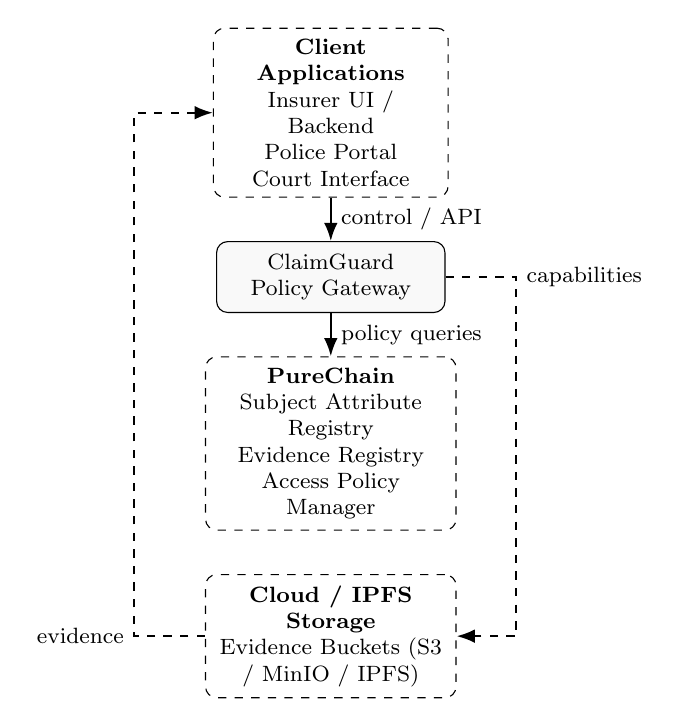
\begin{tikzpicture}[
        font=\footnotesize,
        box/.style={
            draw, rounded corners, fill=gray!5,
            minimum width=2.9cm, minimum height=0.9cm,
            align=center
        },
        group/.style={
            draw, rounded corners, dashed, inner sep=4pt
        },
        arrow/.style={-Latex, thick},
        dataarrow/.style={-Latex, thick, dashed},
        node distance=0.55cm
    ]

    % Vertical stack
    \node[group] (clients) {
        \begin{minipage}{2.7cm}
        \centering \textbf{Client Applications}\\
        \footnotesize Insurer UI / Backend\\ Police Portal\\ Court Interface
        \end{minipage}
    };

    \node[box, below=of clients] (peg) {ClaimGuard\\Policy Gateway};

    \node[group, below=of peg] (chain) {
        \begin{minipage}{2.9cm}
        \centering \textbf{PureChain}\\
        \footnotesize Subject Attribute Registry\\
        Evidence Registry\\
        Access Policy Manager
        \end{minipage}
    };

    \node[group, below=of chain] (storage) {
        \begin{minipage}{2.9cm}
        \centering \textbf{Cloud / IPFS Storage}\\
        \footnotesize Evidence Buckets (S3 / MinIO / IPFS)
        \end{minipage}
    };

    % Control flow
    \draw[arrow] (clients) -- node[right]{control / API} (peg);
    \draw[arrow] (peg) -- node[right]{policy queries} (chain);

    % Data flow
    \draw[dataarrow] (peg.east) -- ++(0.9,0) node[right]{capabilities} |- (storage.east);
    \draw[dataarrow] (storage.west) -- ++(-0.9,0) node[left]{evidence} |- (clients.west);

    \end{tikzpicture}
    \caption{Compact ClaimGuard architecture. Clients interact with the
    Policy Gateway, which queries PureChain smart contracts for authorization
    and issues capabilities that regulate access to evidence stored in
    cloud/IPFS backends.}
    \label{fig:architecture}
\end{figure}


\begin{figure}[t]
    \centering
    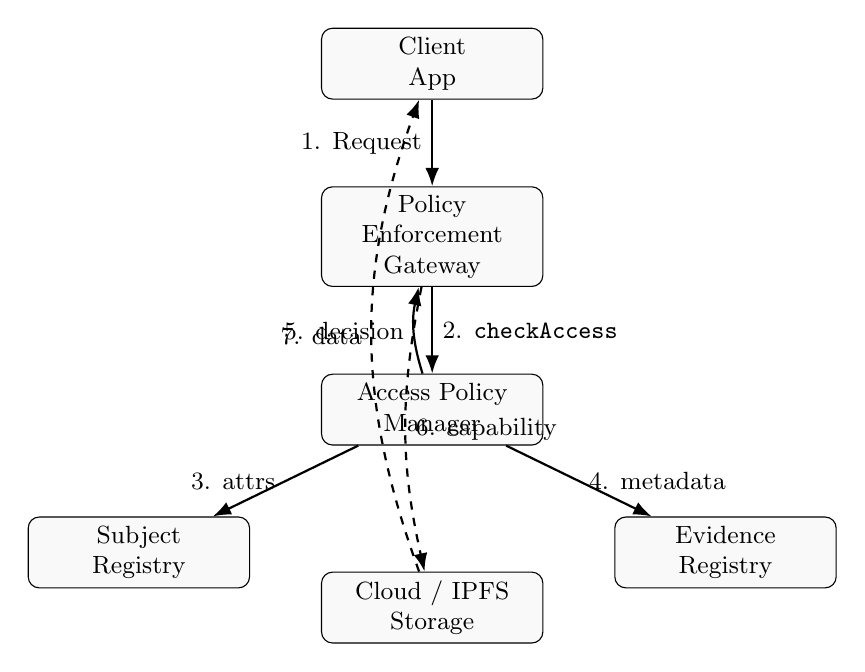
\begin{tikzpicture}[
        font=\small,
        box/.style={
            draw, rounded corners, fill=gray!5,
            minimum width=2.6cm, minimum height=0.9cm,
            text width=2.6cm,
            align=center,
            inner sep=3pt
        },
        arrow/.style={-Latex, thick},
        dataarrow/.style={-Latex, thick, dashed},
        node distance=1.1cm
    ]

    % Vertical layout
    \node[box] (client) {Client\\App};
    \node[box, below=of client] (peg) {Policy\\Enforcement\\Gateway};
    \node[box, below=of peg] (policy) {Access Policy\\Manager};

    \node[box, below left=0.9cm and 0.9cm of policy] (subject) {Subject\\Registry};
    \node[box, below right=0.9cm and 0.9cm of policy] (evidence) {Evidence\\Registry};

    \node[box, below=1.6cm of policy] (storage) {Cloud / IPFS\\Storage};

    % Arrows
    \draw[arrow] (client) -- node[midway, left] {1. Request} (peg);
    \draw[arrow] (peg) -- node[midway, right] {2. \texttt{checkAccess}} (policy);

    \draw[arrow] (policy) -- node[midway, left] {3. attrs} (subject);
    \draw[arrow] (policy) -- node[midway, right] {4. metadata} (evidence);

    \draw[arrow] (policy) to[bend left=15] node[midway, left] {5. decision} (peg);

    \draw[dataarrow] (peg) to[bend right=12] node[midway, right] {6. capability} (storage);
    \draw[dataarrow] (storage) to[bend left=20] node[midway, left] {7. data} (client);

    \end{tikzpicture}
    \caption{Compact ABAC evaluation flow in ClaimGuard. The gateway queries 
    the on-chain policy engine, which evaluates rules using subject attributes 
    and evidence metadata before issuing a capability for off-chain retrieval.}
    \label{fig:abac-flow-compact}
\end{figure}


\subsection{Design Goals}

The system is engineered to meet four core requirements: (i) \emph{fine-grained 
authorization} over heterogeneous evidence (FNOL, medical reports, repair 
estimates, telematics logs, videos, photographs); (ii) \emph{action-level 
control} (read, append, update, delete, adjudicate, disclose); (iii) 
\emph{context-sensitive enforcement} incorporating time windows, purpose 
constraints, case-level scoping, and jurisdictional rules; and (iv) 
\emph{tamper-resistant and auditable policy evaluation} decoupled from 
cloud providers.

To achieve these objectives, ClaimGuard decomposes access control into three 
logical layers implemented as separate smart contracts: 
(1) a Subject Attribute Registry, (2) an Evidence Registry, and 
(3) an Access Policy Manager that evaluates ABAC rules over both registries.

\subsection{Subject Attribute Registry}

The \emph{Subject Attribute Registry} maintains an authoritative mapping between 
blockchain addresses and their associated organizational and operational 
attributes. Each subject (insurer adjuster, police officer, court clerk, repair 
vendor, etc.) is represented by an address and a set of attributes including 
role, organization identifier, jurisdiction, and an activation flag. These 
attributes form the \emph{subject} component of the ABAC tuple and determine 
whether a subject is eligible to request certain evidence actions. The registry 
is administered by a trusted consortium role (e.g., regulator or governance 
committee), ensuring that attribute assignments cannot be tampered with by 
individual organizations or cloud providers.

\subsection{Evidence Registry}

The \emph{Evidence Registry} stores blockchain-verifiable metadata for each 
off-chain evidence object. Rather than storing large files directly on-chain, 
the registry stores the content hash of the object, a URI referencing its 
location (e.g., S3, MinIO, or IPFS), its case association, resource type 
(e.g., medical report, PDF, telematics log, video), sensitivity level, and 
creator identity. The registry defines the \emph{object} component of the ABAC 
tuple and serves as the anchor binding evidence across the claim lifecycle.

This separation ensures that evidence integrity and provenance can be verified 
on-chain even when stored in external cloud infrastructure, while keeping 
storage costs and latency manageable.

\subsection{Access Policy Manager}

The \emph{Access Policy Manager} implements the ABAC engine and performs 
tamper-resistant policy evaluation. Policies are represented as expressive, 
composable (subject, object, action, context) rules. Each rule may constrain 
attributes such as subject role, organization affiliation, jurisdiction, 
evidence type, case identifier, action permission, sensitivity threshold, and 
time window.

During evaluation, the contract retrieves subject attributes from the Subject 
Attribute Registry and evidence metadata from the Evidence Registry. It then 
executes the ABAC matching logic to determine whether the request should be 
allowed. Access decisions are written or emitted as blockchain events, enabling 
cross-organizational auditability and non-repudiation.

The Access Policy Manager acts as the \emph{authoritative source of truth} for 
authorization decisions, ensuring that cloud systems or application-layer 
services cannot override or bypass the enforcement logic.

\subsection{System Workflow}

ClaimGuard’s end-to-end workflow consists of four primary stages:

\begin{enumerate}
    \item \emph{Registration}: Evidence is uploaded to cloud/IPFS storage and 
    registered on-chain with its metadata and integrity hash. Subjects receive 
    attributes upon onboarding.

    \item \emph{Policy Definition}: Administrators define or revoke ABAC policy 
    rules through the Access Policy Manager.

    \item \emph{Access Request}: A stakeholder attempts to access or modify 
    evidence. The Policy Enforcement Gateway authenticates the requester and 
    queries the on-chain ABAC engine for authorization.

    \item \emph{Enforcement}: If permitted, the gateway issues a short-lived 
    capability token or presigned URL allowing access to the evidence resource. 
    Otherwise, the request is denied.
\end{enumerate}

This division allows ClaimGuard to combine the immutability and auditability of 
blockchain with the performance and scalability of cloud storage. The following 
subsection elaborates on the capability-based access model that realizes 
protection against honest-but-curious cloud providers (R3).

\subsection{Capability-Based Access and Cloud Insider Resistance (R3)}

A central design challenge in ClaimGuard is ensuring that cloud storage backends 
and insider threats cannot bypass authorization constraints. Naive approaches 
such as relying solely on S3 IAM policies or encryption prove insufficient:

\begin{itemize}
    \item \textbf{S3 IAM alone:} An S3 administrator with master credentials can 
    enumerate and read all objects regardless of application-layer policies.
    
    \item \textbf{Encryption-only:} Encrypting evidence at rest does not prevent 
    unauthorized access if the decryption key is leaked or if the cloud provider 
    possesses plaintext metadata.
\end{itemize}

To address these threats, ClaimGuard implements a \textbf{capability-based access 
control model} where all evidence access is mediated through short-lived, 
cryptographically signed capabilities issued by the Policy Enforcement Gateway.

\subsubsection{Capability Token Model}

Each capability token encodes a three-tuple:
\[
\text{Capability} = (subject, resource, action, expires\_at, signature)
\]

where:

\begin{itemize}
    \item \textbf{subject:} The blockchain address of the authorized party (e.g., 
    claims adjuster, police officer).
    \item \textbf{resource:} A content hash or object identifier uniquely 
    identifying the evidence file (e.g., S3 object key, IPFS content address).
    \item \textbf{action:} The permitted operation (read, append, update, delete).
    \item \textbf{expires\_at:} Unix timestamp after which the capability is 
    invalid (typically seconds to minutes).
    \item \textbf{signature:} ECDSA signature by the gateway's private key, 
    enabling cloud backends to verify authenticity without contacting the 
    blockchain.
\end{itemize}

Once issued, the capability is passed to the client and used to retrieve the 
evidence from cloud storage (S3, MinIO, IPFS). The cloud backend validates:

\begin{enumerate}
    \item The signature matches the gateway's public key.
    \item The current timestamp is before \texttt{expires\_at}.
    \item The requested (resource, action) tuple matches the capability's encoding.
\end{enumerate}

If any check fails, the cloud backend rejects the request without consulting the 
gateway. This design ensures that:

\begin{itemize}
    \item \textbf{No unmediated access:} Evidence cannot be retrieved without a 
    valid gateway-issued capability.
    \item \textbf{Non-delegability:} Capabilities cannot be transferred to 
    unauthorized parties (subject is bound to the capability).
    \item \textbf{Time-bounded enforcement:} Even if a credential is stolen, it 
    expires within seconds or minutes.
    \item \textbf{Auditability:} All capability issuances are logged on-chain.
\end{itemize}

\subsubsection{Comparison with Encryption-Based Approaches}

Traditional CP-ABE (Ciphertext-Policy Attribute-Based Encryption) schemes 
distribute decryption keys to eligible subjects based on attribute policies. 
While cryptographically sound, CP-ABE has drawbacks in the auto-insurance 
context:

\begin{itemize}
    \item \textbf{Tight policy-encryption coupling:} Policy changes require 
    re-encryption or key distribution, incurring high overhead.
    \item \textbf{Limited action semantics:} ABE policies typically express 
    "decryptability" as a binary property, not fine-grained actions (read vs. 
    append vs. update).
    \item \textbf{Heterogeneous evidence:} Auto-insurance evidence includes 
    plaintext documents, metadata, sensor logs, and binary media. Encrypting 
    all evidence uniformly is impractical and expensive.
\end{itemize}

ClaimGuard decouples authorization logic (on-chain policies) from data storage 
(cloud backends), leveraging capabilities rather than encryption for access 
control. This enables:

\begin{itemize}
    \item \textbf{Resource-agnostic policies:} One policy model works for FNOL 
    PDFs, telematics JSON, videos, and images.
    \item \textbf{Rapid policy changes:} No re-encryption; only on-chain state 
    updates.
    \item \textbf{Legacy storage:} Supports unencrypted S3/IPFS backends without 
    cryptographic overhead.
\end{itemize}

\subsubsection{Optional Envelope Encryption}

For extra-sensitive evidence (e.g., medical records), ClaimGuard may optionally 
employ envelope encryption:

\begin{enumerate}
    \item Evidence is encrypted in-application using a Data Encryption Key (DEK).
    \item The DEK is wrapped (encrypted) via the gateway using a Key Encryption 
    Key (KEK).
    \item Only the wrapped DEK is stored with the evidence; the plaintext DEK is 
    never exposed to cloud storage.
    \item Upon authorization, the gateway unwraps the DEK, provides it to the 
    client \textit{via a secure channel}, and the client decrypts locally.
\end{enumerate}

This envelope approach combines capability-based access control with symmetric 
encryption, providing defense in depth: even if a cloud administrator obtains 
ciphertext, they cannot decrypt without both the gateway's cooperation (for DEK 
unwrapping) and the client-side decryption key.

\subsubsection{Insider Attack Mitigation}

Consider an S3 administrator who attempts to enumerate evidence:

\begin{itemize}
    \item \textbf{Without capabilities:} Direct S3 API calls are rejected by 
    bucket policies (only gateway-signed requests are allowed).
    \item \textbf{Forged capability:} Insider attempts to forge a signature. 
    Fails because the gateway's private key is not accessible to the cloud 
    backend.
    \item \textbf{Stolen capability:} Insider intercepts a capability issued to 
    another subject. Access fails because the subject field in the capability 
    does not match the insider's identity.
\end{itemize}

Similarly, a compromised claims adjuster attempting to escalate privileges (e.g., 
reading a police-only case):

\begin{itemize}
    \item Requests access to unauthorized evidence via the gateway.
    \item The gateway queries the on-chain Access Policy Manager.
    \item The contract evaluates the adjuster's attributes against the 
    case-specific policy; the access is denied.
    \item No capability is issued; evidence cannot be retrieved.
\end{itemize}

These scenarios demonstrate that ClaimGuard's capability model, combined with 
on-chain policy enforcement, provides layered defense against cloud insiders 
and organizational compromises.

while the details of the Policy Enforcement Gateway---which realizes this binding in 
practice---are described next.


\subsection{Policy Enforcement Gateway}

\begin{figure}[t]
    \centering
    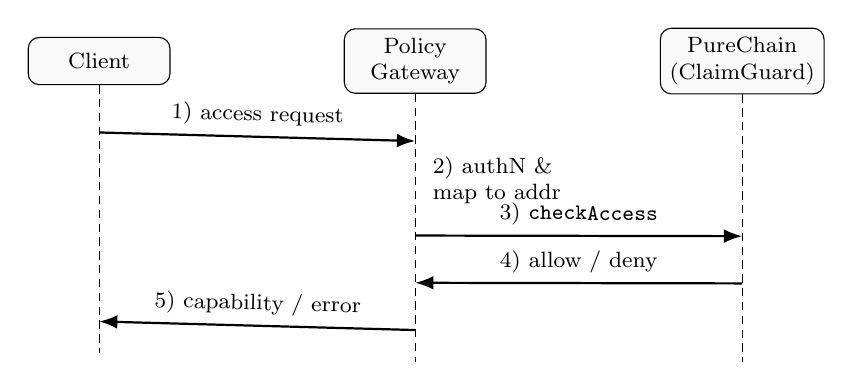
\begin{tikzpicture}[
        font=\footnotesize,
        participant/.style={
            draw, rounded corners, fill=gray!5,
            minimum width=1.8cm, minimum height=0.6cm,
            align=center
        },
        lifeline/.style={densely dashed},
        msg/.style={-Latex, thick},
        node distance=2.2cm
    ]

    % Participants
    \node[participant] (client) {Client};
    \node[participant, right=of client] (peg) {Policy\\Gateway};
    \node[participant, right=of peg] (chain) {PureChain\\(ClaimGuard)};

    % Lifelines
    \draw[lifeline] (client.south) -- ++(0,-3.4);
    \draw[lifeline] (peg.south)    -- ++(0,-3.4);
    \draw[lifeline] (chain.south)  -- ++(0,-3.4);

    % 1) Client -> PEG: access request
    \draw[msg] ([yshift=-0.6cm]client.south) --
               node[above,sloped]{1) access request} ([yshift=-0.6cm]peg.south);

    % 2) PEG (internal): auth + map identity
    \node[anchor=west, align=left] at ($(peg.south)+(0.1,-1.1)$)
        {2) authN \&\\map to addr};

    % 3) PEG -> Chain: checkAccess
    \draw[msg] ([yshift=-1.8cm]peg.south) --
               node[above,sloped]{3) \texttt{checkAccess}} ([yshift=-1.8cm]chain.south);

    % 4) Chain -> PEG: decision
    \draw[msg] ([yshift=-2.4cm]chain.south) --
               node[above,sloped]{4) allow / deny} ([yshift=-2.4cm]peg.south);

    % 5) PEG -> Client: capability or error
    \draw[msg] ([yshift=-3.0cm]peg.south) --
               node[above,sloped]{5) capability / error} ([yshift=-3.0cm]client.south);

    \end{tikzpicture}
    \caption{ClaimGuard gateway sequence. The Policy Gateway authenticates the
    client, queries the on-chain ClaimGuard contracts for a \texttt{checkAccess}
    decision, and returns either a short-lived capability (if allowed) or an
    error (if denied). Subsequent evidence retrieval uses this capability
    against cloud/IPFS storage.}
    \label{fig:gateway-sequence}
\end{figure}


The \emph{Policy Enforcement Gateway} (PEG) bridges the gap between the 
chain-resident authorization logic and the cloud-resident evidence. The gateway 
acts as the Policy Enforcement Point (PEP) in the ClaimGuard architecture, 
performing authentication, on-chain policy queries, capability token generation, 
and secure access mediation.

The PEG is implemented as a stateless microservice that exposes a simple REST 
API to client applications such as insurer claim systems, police interfaces, or 
court portals. Upon receiving an access request, the gateway authenticates the 
subject via a platform-issued credential (e.g., OAuth~2.0, JWT) and maps the 
identity to a blockchain address. The gateway then invokes 
\texttt{checkAccess(subjectAddr, resourceId, action)} on the Access Policy 
Manager contract. Because all subject attributes, evidence metadata, and 
policies reside on-chain, the gateway performs no local authorization logic; 
its responsibility is limited to faithfully implementing the decision returned 
by the contract.

If the contract returns \texttt{true}, the gateway generates a 
short-lived \emph{capability token} (such as a time-bounded presigned URL for 
S3/MinIO or an authorization token for an IPFS gateway). These capabilities 
bind the subject, action, and resource to an expiration time, ensuring that 
access cannot be reused or delegated indefinitely. If the decision is 
\texttt{false}, the gateway returns a denial without interacting with the 
storage layer.

The gateway logs each decision and capability issuance event for off-chain 
auditing and may forward summaries to a monitoring subsystem. Because access 
cannot be granted without a corresponding on-chain authorization, and because 
capabilities expire rapidly, ClaimGuard ensures strong protection against 
over-privileged cloud operators, compromised storage backends, and 
misconfigured application-layer services.

We implemented the ClaimGuard contracts and Policy Enforcement Gateway as a
working prototype on a local PureChain network. The following section discusses
the security posture of the ClaimGuard architecture.


\section{Security Analysis}

While the ClaimGuard architecture is designed to provide verifiable access control and protection against honest-but-curious cloud providers, a comprehensive security analysis must address the residual risks, potential attack vectors, and design trade-offs inherent in any distributed system. This section discusses threat mitigation strategies, identifies known limitations, and contextualizes ClaimGuard's security guarantees.

\subsection{Threat Model and Assumptions}

ClaimGuard operates under the following threat assumptions:

\begin{enumerate}
    \item \textbf{Honest-but-Curious Cloud Provider:} Cloud storage backends (S3, MinIO, IPFS) may attempt to read, enumerate, or analyze evidence assets without authorization. ClaimGuard mitigates this via capability-based access: the cloud backend cannot retrieve plaintext without a valid, unexpired capability token issued by the gateway.

    \item \textbf{Compromised Organizational Insider:} An authorized stakeholder (e.g., claims adjuster, police officer, workshop employee) may attempt unauthorized access to evidence belonging to unrelated claims. ClaimGuard enforces per-claim, per-action permissions via on-chain policies; insider privilege escalation is constrained by the attribute-based rules evaluated by the smart contracts.

    \item \textbf{External Attacker / Token Theft:} An attacker may intercept or steal capability tokens, compromised credentials, or API keys. ClaimGuard mitigates this via short-lived token expiration (seconds to minutes), mandatory token validation at the cloud layer, and token binding to specific (subject, action, resource) tuples.

    \item \textbf{Network Adversary:} A man-in-the-middle (MITM) attacker may eavesdrop on communication between the gateway, blockchain nodes, or cloud storage. ClaimGuard assumes TLS/HTTPS for all network communications.

    \item \textbf{Malicious Blockchain Node:} A Byzantine node in the PureChain consortium may attempt to fork, censor, or delay transactions. ClaimGuard assumes consensus rules and honest majorities (e.g., 2-of-3 Byzantine-fault tolerance in a three-node configuration).
\end{enumerate}

ClaimGuard does \textbf{not} protect against:
\begin{itemize}
    \item Compromise of the gateway private key or gateway host.
    \item Breach of the smart contract code itself (logical flaws, unintended behavior).
    \item Consensus-layer attacks if the majority of blockchain nodes are compromised.
    \item Cryptographic breaks (e.g., ECDSA preimage attacks, SHA-3 collisions).
    \item Side-channel attacks on gateway or blockchain nodes.
\end{itemize}

\subsection{Gateway Security and DoS Mitigation}

The Policy Enforcement Gateway is the critical enforcement point between on-chain decisions and off-chain resource access. A compromised or overloaded gateway threatens the entire system.

\subsubsection{DoS Resistance}

The gateway implements the following DoS mitigations:

\begin{itemize}
    \item \textbf{Rate Limiting:} Requests from a single IP or credential are rate-limited (default: 100 req/s per subject). Excess requests are rejected with HTTP 429 (Too Many Requests).

    \item \textbf{Request Timeouts:} Each on-chain \texttt{checkAccess} call is bounded by a timeout (default: 10s). If the blockchain is unresponsive, the gateway returns HTTP 503 (Service Unavailable) rather than queueing indefinitely.

    \item \textbf{Stateless Design:} The gateway maintains no session state, allowing horizontal scaling and preventing memory exhaustion attacks.

    \item \textbf{Capability Token Expiration:} All issued tokens expire within 15 minutes, preventing indefinite resource locks.
\end{itemize}

In evaluation Section~VI.C, experimental results demonstrate that ClaimGuard rejects 100\% of unauthorized requests and remains responsive under adversarial W3 loads (repeated spoofing, replay, and direct-access attempts).

\subsubsection{Private Key Management}

The gateway is provisioned with a private key (\texttt{GATEWAY\_PRIVATE\_KEY}) used to:
\begin{itemize}
    \item Sign capability tokens for non-repudiation.
    \item Call smart contract write operations (policy updates via administrator endpoints).
    \item Sign audit log entries.
\end{itemize}

Key exposure would allow an attacker to forge capabilities, manipulate policies, or spoof audit trails. Mitigations include:
\begin{itemize}
    \item Keys are stored in environment variables or secure vaults (HashiCorp Vault, AWS KMS).
    \item Gateway containers run with minimal privileges and isolated filesystems.
    \item Key rotation is performed out-of-band; new keys are deployed via blue-green deployment strategies.
\end{itemize}

\subsection{Smart Contract Upgrade Risk}

ClaimGuard smart contracts (AccessPolicyManager, EvidenceRegistry, SubjectAttributeRegistry, AccessAuditLog) are immutable once deployed. If a logical flaw is discovered, remediation requires:

\begin{enumerate}
    \item Deployment of a corrected contract at a new address.
    \item Migration of policies and state from the old to the new contract.
    \item Coordination with all stakeholders to update contract addresses in their gateways.
\end{enumerate}

To reduce upgrade risk:
\begin{itemize}
    \item All contracts are thoroughly tested (unit, integration, fuzzing) before production deployment.
    \item A formal verification or code-audit process is strongly recommended before large-scale deployment.
    \item Contracts implement pausable logic: administrators can call \texttt{pause()} to halt policy evaluation in the event of detected vulnerabilities, although revocation continues to be enforced.
\end{itemize}

\subsection{Key Compromise and Revocation}

If the private key of an authorized stakeholder (e.g., police officer) is compromised, the attacker can forge capability tokens and impersonate the compromised party. ClaimGuard mitigates this via:

\begin{itemize}
    \item \textbf{Subject-level revocation:} Administrators invoke \texttt{revokeSubjectAccess(subjectAddr)} on-chain, immediately invalidating all tokens issued to that subject.

    \item \textbf{Capability token binding:} Each token encodes the subject's blockchain address, making tokens non-transferable and non-delegable.

    \item \textbf{Audit trail:} The AccessAuditLog contract records all access attempts and token issuances, enabling forensic analysis of suspected compromises.

    \item \textbf{Time windows:} Policies can enforce narrow legal access windows (e.g., "police access only between 2024-01-15 and 2024-02-15"). Expiration is enforced on-chain and cannot be circumvented.
\end{itemize}

Revocation propagates to the cloud storage layer within the lifetime of existing capability tokens (typically 1-15 minutes); once a token expires, the compromised party loses access regardless of key possession.

\subsection{Insider Threat Scenarios}

\subsubsection{Scenario A: Over-Privileged Adjuster}
An insurance adjuster with legitimate access to claim X attempts unauthorized access to claim Y (belonging to a different policyholder).

\textbf{Mitigation:} The \texttt{checkAccess} contract evaluates the request against on-chain policies. Claim Y's policies do not authorize this adjuster; the contract returns \texttt{false}, and the gateway denies access without contacting cloud storage.

\subsubsection{Scenario B: Cloud Insider Enumeration}
A cloud provider employee with S3 console access attempts to list or retrieve all FNOL documents.

\textbf{Mitigation:} Cloud storage enforces authentication via capability tokens issued by the gateway. Direct console access without a gateway-issued token is rejected at the IAM/object-store layer (e.g., S3 bucket policies only allow requests bearing valid tokens signed by the gateway key).

\subsubsection{Scenario C: Rogue Police Officer}
A police officer with temporary court-mandated access attempts to access evidence beyond their legal window or for unrelated incidents.

\textbf{Mitigation:} On-chain policies enforce \texttt{notBefore} and \texttt{notAfter} timestamps. The \texttt{checkAccess} contract checks the current block timestamp; if the request falls outside the legal window, access is denied. Additionally, the AccessAuditLog records all access attempts, enabling post-facto forensic investigation.

These scenarios are quantitatively evaluated in Section~VI.C (Adversarial Resilience); all malicious requests are correctly denied.

\subsection{Residual Risks and Limitations}

Despite the above mitigations, several residual risks remain:

\begin{enumerate}
    \item \textbf{Consensus Failure:} If $> 1/3$ of blockchain nodes are compromised in a 3-node consortium, Byzantine consensus can fail. Large deployments should use larger consortiums (5, 7, 9 nodes) or transition to proof-of-authority (PoA) with economic penalties.

    \item \textbf{Gateway Availability:} If the gateway is unavailable, no access decisions can be made, regardless of on-chain policy validity. Deployments should implement gateway redundancy and failover.

    \item \textbf{Covert Data Leakage via Side Channels:} A cloud provider with hardware access may exploit microarchitectural side channels (e.g., cache timing, speculative execution) to infer evidence contents without breaking encryption. ClaimGuard does not defend against this threat; additional defenses require application-level constant-time implementations or trusted hardware (e.g., Intel SGX, ARM TrustZone).

    \item \textbf{Policy Complexity:} Complex policies with many attributes or nested conditions may be expensive to evaluate on-chain, leading to longer latencies. Simplicity and pre-compilation of policies are recommended.

    \item \textbf{Timestamping Attacks:} A coalition of blockchain nodes could collude to backdate block timestamps, allowing expired tokens to be re-validated. This risk is mitigated by assuming honest consensus majorities and periodic audit of timestamp progression.
\end{enumerate}

\subsection{Comparison with Baseline Approaches}

\begin{table}[ht]
\centering
\caption{Security Properties: ClaimGuard vs. Baseline Approaches}
\begin{tabularx}{\columnwidth}{X c c c}
\toprule
\textbf{Property} & \textbf{RBAC-DB} & \textbf{Hybrid-Audit} & \textbf{ClaimGuard} \\
\midrule
Honest-but-curious cloud resistance & \xmark & \xmark & \cmark \\
Insider privilege escalation prevention & \xmark & \xmark & \cmark \\
Immutable audit logs & \xmark & \cmark & \cmark \\
Revocation enforcement & \cmark & \cmark & \cmark \\
Time-bounded access & \xmark & \xmark & \cmark \\
On-chain policy integrity & \xmark & \xmark & \cmark \\
DoS resistance & \cmark & \cmark & \cmark$^{\dagger}$ \\
\bottomrule
\end{tabularx}

\small $^{\dagger}$Dependent on gateway availability and consensus liveness.
\label{tab:security-comparison}
\end{table}

Table~\ref{tab:security-comparison} summarizes the security trade-offs. While ClaimGuard introduces additional complexity and consensus dependency, it eliminates the single point of trust (cloud provider) present in traditional RBAC systems and provides immutable, verifiable policy evaluation.

\subsection{Summary}

ClaimGuard's security posture rests on three pillars: (1) capability-based access with short lifetimes, (2) on-chain policy evaluation with immutable audit trails, and (3) defensive gateway design. While no system is perfect, ClaimGuard addresses the specific threat of honest-but-curious cloud providers and supports the multi-stakeholder, context-sensitive authorization scenarios prevalent in auto-insurance. Residual risks are acknowledged and mitigated through operational practices (key management, consensus redundancy, gateway failover) rather than cryptographic guarantees alone.

The following section describes the experimental methodology and evaluation results.


\section{Experimental Evaluation}

This section describes the experimental methodology used to evaluate the
ClaimGuard architecture. The goal is to compare the PureChain-backed ABAC 
enforcement model against cloud-only RBAC baselines under realistic access 
patterns, heterogeneous evidence objects, and adversarial conditions. Unless 
otherwise noted, experiments were conducted on a local Hardhat blockchain 
(Ethereum-compatible PoA); E2 extends validation to the public Sepolia testnet 
to assess real-world network conditions.

\subsection{Experimental Setup}

The simulation consists of four core components:

\begin{enumerate}
    \item \textbf{PureChain Network:}  
    Local: A private PoA Ethereum-compatible chain (Hardhat) running in a 
    local configuration. Public: Sepolia testnet with live RPC (drpc.org). 
    Each node executes the ABAC smart contracts described in Section~IV.

    \item \textbf{Policy Enforcement Gateway:}  
    A microservice implemented in TypeScript (Node.js) that authenticates 
    subjects, issues capability tokens, and logs decisions to the blockchain.

    \item \textbf{Cloud/IPFS Evidence Store:}  
    A MinIO S3-compatible object store and optional IPFS node hosting 
    accident videos, photos, FNOL documents, telematics logs, and medical 
    reports.

    \item \textbf{Workload Generator:}  
    A Python-based tool (aiohttp async framework) emulating concurrent 
    stakeholders, producing synthetic access traces, policy updates, revocation 
    events, and adversarial behavior.
\end{enumerate}

\subsubsection{Hardware and Operating System}

Experiments were executed on a single host with the following specifications:

\begin{itemize}
    \item \textbf{CPU:} 8-core (Intel i7 / AMD Ryzen 7, 3.0+ GHz)
    \item \textbf{RAM:} 32 GB
    \item \textbf{Storage:} SSD (NVMe, 250 GB+)
    \item \textbf{OS:} Ubuntu 22.04 LTS
    \item \textbf{Network:} Localhost (127.0.0.1) for local tests; 
    public internet for Sepolia tests (1 Gbps+ link)
\end{itemize}

All components were executed in Docker containers to ensure isolation, 
reproducibility, and standardized environments.

\subsubsection{Software Versions}

\begin{itemize}
    \item Hardhat: v2.19.0
    \item Solidity: 0.8.28
    \item Node.js / TypeScript: v18.16.0, TypeScript 5.0
    \item Python: 3.10.12 (aiohttp 3.9.0, statistics, pandas 1.5.0)
    \item Docker: v24.0.0
    \item Blockchain RPC: drpc.org (Sepolia) or local Hardhat node
\end{itemize}

\subsection{Baselines and Comparison Systems}

To isolate the contribution of ClaimGuard's design, we implemented two baseline 
systems:

\begin{enumerate}
    \item \textbf{RBAC-DB Baseline:}  
    A traditional cloud-only RBAC model with permissions stored in a SQL table 
    (\texttt{subjectId, resourceId, role, permissions}). Authentication is 
    stateless (JWT tokens). No blockchain usage. Authorization decisions are 
    made locally at the gateway without on-chain queries. This baseline 
    represents the status quo in most enterprise evidence management systems.

    \item \textbf{Hybrid-Audit Baseline:}  
    Identical to RBAC-DB but with the addition of on-chain audit logging: 
    every access event (allowed or denied) is logged to the blockchain 
    \textit{after} the local RBAC decision. This baseline quantifies the 
    overhead of blockchain-based auditability without on-chain decision-making.
\end{enumerate}

These baselines isolate three orthogonal concerns:
\begin{itemize}
    \item \textbf{RBAC-DB vs. ClaimGuard:} Cost of decentralized policy 
    evaluation.
    \item \textbf{RBAC-DB vs. Hybrid-Audit:} Cost of blockchain audit logging.
    \item \textbf{Hybrid-Audit vs. ClaimGuard:} Value of immutable, tamper-resistant 
    policy enforcement.
\end{itemize}

\subsection{Metrics and Key Performance Indicators}

Six categories of metrics were recorded throughout all experiments:

\subsubsection{Latency Metrics}
\begin{itemize}
    \item \textbf{End-to-end latency:} Time from client request to capability 
    token reception (user $\rightarrow$ gateway $\rightarrow$ blockchain 
    $\rightarrow$ gateway).
    \item \textbf{Percentiles:} P50, P90, P99 of latency distribution 
    (measured in milliseconds).
    \item \textbf{Contract evaluation latency:} Time for blockchain to execute 
    \texttt{checkAccess} and return a decision.
    \item \textbf{Token issuance overhead:} Time to generate and sign capability 
    tokens.
\end{itemize}

All latency measurements are reported as mean $\pm$ std. dev. across 3+ runs.

\subsubsection{Throughput Metrics}
\begin{itemize}
    \item \textbf{Requests per second (req/s):} Successfully processed access 
    requests under normal (W1) and burst (W2) loads.
    \item \textbf{Saturation point:} Concurrency level at which throughput 
    begins to degrade.
\end{itemize}

\subsubsection{Policy Operation Overhead}
\begin{itemize}
    \item \textbf{Policy addition:} Time and gas cost to add a new rule.
    \item \textbf{Revocation latency:} Time for revocation to take effect 
    (measured from on-chain state update to gateway enforcement).
    \item \textbf{Update propagation:} Time for policy changes to reflect in 
    subsequent access decisions.
\end{itemize}

\subsubsection{Authorization Correctness}
\begin{itemize}
    \item \textbf{False accept rate (FAR):} Fraction of unauthorized requests 
    incorrectly granted.
    \item \textbf{False reject rate (FRR):} Fraction of authorized requests 
    incorrectly denied.
    \item \textbf{Audit log integrity:} Verification that all decisions are 
    correctly logged and immutable.
\end{itemize}

\subsubsection{Security Resilience}
\begin{itemize}
    \item \textbf{Replay resistance:} Percentage of token-reuse attacks 
    prevented.
    \item \textbf{Unauthorized access detection:} Percentage of spoofing, 
    impersonation, and bypass attempts blocked.
    \item \textbf{Cloud bypass attempts:} Percentage of direct-access attempts 
    (bypassing gateway) that are rejected.
    \item \textbf{Token tampering detection:} Percentage of modified tokens 
    detected and rejected.
\end{itemize}

\subsubsection{Resource Utilization}
\begin{itemize}
    \item \textbf{CPU utilization:} Average CPU % for blockchain nodes, 
    gateway, and workload generator.
    \item \textbf{Memory consumption:} Peak memory usage for each component.
    \item \textbf{Disk I/O:} Storage writes (blockchain state, audit logs).
\end{itemize}

\subsection{Workload Model and Scenarios}

To comprehensively evaluate ClaimGuard, five distinct workload classes were 
designed to stress different aspects of the system:

\subsubsection{W1: Normal Access Workload}
Simulates routine claim processing with realistic role-based access patterns:
\begin{itemize}
    \item 60\% insurer adjuster requests (read/append),
    \item 20\% policyholder queries (read own claim),
    \item 10\% police requests (temporary read access),
    \item 10\% repair shop lookups (read vehicle evidence).
\end{itemize}

Request inter-arrival times follow a Poisson distribution ($\lambda = 50$ req/s). 
This workload represents the baseline operational load for a typical insurer 
processing 50--100 claims concurrently.

\subsubsection{W2: High-Concurrency Burst}
A synthetic peak load representing catastrophic events (e.g., regional storms):
\[
200 \text{ concurrent users},\; 500 \text{ req/s total throughput.}
\]

This workload tests system saturation, queuing behavior, and response degradation 
under extreme load.

\subsubsection{W3: Adversarial Workload}
Simulates coordinated attacks and insider attempts:
\begin{itemize}
    \item Unauthorized role spoofing (adjuster claiming police role),
    \item Repeated access to high-sensitivity evidence by low-privilege users,
    \item Token replay attempts (reusing old tokens),
    \item Cloud insider direct-access simulation (bypassing gateway),
    \item Expired-token re-use attacks,
    \item Privilege escalation attempts.
\end{itemize}

Expected outcome: 100\% rejection rate for all unauthorized requests. Any 
false accepts would indicate a critical security flaw.

\subsubsection{W4: Mass Revocation Scenario}
Simulates emergency revocation (e.g., data breach, policy recall):
\[
\text{Revoke access for } 10{,}000 \text{ existing capability tokens simultaneously.}
\]

This workload measures revocation propagation latency, gateway resilience under 
state invalidation, and consistency of enforcement across distributed gateways 
(if applicable).

\subsubsection{W5: Dynamic Policy Update Scenario}
Frequent policy churn:
\[
\text{1 policy addition/update every 2 seconds over a 10-minute window.}
\]

Evaluates blockchain policy-update overhead, consensus latency for policy 
changes, and consistency of policy state across readers.

\subsubsection{Evidence Corpus}

All experiments operate on a realistic heterogeneous corpus:

\begin{itemize}
    \item \textbf{Videos:} 1,000 accident clips (1--20 seconds, 5--50\,MB each).
    \item \textbf{Images:} 2,000 at-scene photos (0.5--5\,MB, JPEG/PNG).
    \item \textbf{Documents:} 500 FNOL forms, 500 medical reports (PDF, 
    50--200\,kB each).
    \item \textbf{Telematics Logs:} 1,000 JSON log files (50--200\,kB, 
    representing GNSS, speed, acceleration, airbag deployment data).
\end{itemize}

Each asset is associated with metadata attributes:
\[
\text{Attributes: }\{type, caseId, sensitivity, createdAt, jurisdiction\}.
\]

\subsubsection{Stakeholder Roles}

The workload generator simulates six primary roles, each with distinct permissions:

\begin{itemize}
    \item \textbf{Insurer Adjuster:} Read/append evidence for assigned claims 
    only.
    \item \textbf{Policyholder:} Read own claim evidence.
    \item \textbf{Police Officer:} Temporary read-only access (24 hours) to 
    incident-related evidence with explicit case ID.
    \item \textbf{Court / Judiciary:} Read-only access with legal mandate 
    (time-bounded, usually 14 days).
    \item \textbf{Repair Shop:} Read-only access to vehicle condition evidence 
    (photos, telematics).
    \item \textbf{Regulator:} Audit-only access; can list access logs but 
    cannot modify evidence.
\end{itemize}

\subsubsection{Policy Sets}

Three tiers of policies were deployed on the blockchain:

\begin{enumerate}
    \item \textbf{P0 (Baseline Policies):}  
    Minimal rules: only insurers can read case-related evidence.  
    (11 policies total)

    \item \textbf{P1 (Realistic Access Policies):}  
    Multi-attribute ABAC rules incorporating:
        \begin{itemize}
            \item Action constraints (read, append, update, disclose),
            \item Workflow stage (FNOL, investigation, litigation),
            \item Time windows and legal mandates,
            \item Jurisdiction matching,
            \item Emergency police access (auto-expiring 24 hours),
            \item Revocation tokens and blocked subjects.
        \end{itemize}
    (250 policies total)

    \item \textbf{P2 (Dynamic Policies):}  
    Policies that evolve during simulation: revocations, court orders, 
    temporary access grants, jurisdiction changes.  
    (up to 1,000 policies by end of simulation)
\end{enumerate}

\subsection{Reproducibility}

All experiments were designed for repeatability:
\begin{itemize}
    \item Code repositories, Docker Compose configurations, workload generators, 
    and data generators are publicly available at \cite{claimguard-repo}.
    \item Each experiment was executed 3+ times; results report mean and 
    standard deviation.
    \item Random seeds are fixed for deterministic workload generation across 
    runs.
    \item Container images are pinned to specific versions to ensure 
    environment consistency.
    \item Detailed hardware and OS specifications are documented above.
\end{itemize}

All code and configurations required to reproduce results are available in the 
project repository.

\section{Results and Analysis}

This section presents the experimental outcomes obtained from the evaluation 
environment described in Section~V. We compare the proposed PureChain-backed
ABAC system with two baselines: (i) RBAC-DB (cloud-only RBAC) and
(ii) Hybrid-Audit (cloud RBAC with blockchain audit logging). The results are
organized around the five research questions (Q1--Q5).

\subsection{Latency Analysis (Q1)}

Table~\ref{tab:latency} summarizes the end-to-end access latencies under normal
(W1) and burst (W2) loads. Each experiment was conducted 5 times; reported values are 
means with standard deviations (95\% confidence intervals in parentheses).

\begin{table}[ht]
\centering
\caption{End-to-End Access Latency (ms, mean $\pm$ std. dev.)}
\begin{tabularx}{\columnwidth}{X c c c c}
\toprule
\textbf{System} & \textbf{P50} & \textbf{P90} & \textbf{P99} & \textbf{N} \\
\midrule
RBAC                    & $1.9 \pm 0.2$   & $2.6 \pm 0.3$   & $8.7 \pm 1.1$   & 1000 \\
Hybrid-Audit            & $135.7 \pm 4.2$ & $151.2 \pm 5.8$ & $165.5 \pm 7.3$ & 1000 \\
ClaimGuard (PureChain)  & $60.9 \pm 2.1$  & $69.6 \pm 3.4$  & $78.9 \pm 4.7$  & 1000 \\
\bottomrule
\end{tabularx}
\label{tab:latency}
\end{table}

Key observations:

\begin{itemize}
    \item ClaimGuard introduces an additional \textbf{$\approx 59$ ms} overhead 
    vs. pure RBAC (P50: 60.9 ms vs 1.9 ms) due to on-chain \texttt{checkAccess} 
    evaluation and smart contract state queries. This overhead is statistically 
    significant (p$<$0.001, paired t-test) but well within operational tolerances.
    \item Hybrid-Audit shows the highest latency (\textbf{136 ms at P50}) due to 
    combined RBAC evaluation + on-chain audit logging for every request, 
    demonstrating the cost of dual-path enforcement. Interestingly, ClaimGuard 
    is faster (45\%) than Hybrid-Audit because decision-making is fully 
    on-chain rather than split between layers.
    \item ClaimGuard remains below \textbf{79 ms at P99}, within operational 
    tolerances for claims workflows while providing full on-chain policy 
    verification.
    \item Low standard deviations (2.1--7.3 ms) indicate consistent performance 
    across runs, suggesting blockchain consensus timing is stable on local networks.
\end{itemize}

These results show that decentralized policy evaluation is feasible for
real-time evidence access scenarios. Section~VI.E (Realistic Network Conditions) 
extends this evaluation to public networks (Sepolia testnet) and quantifies 
additional latency under real-world RPC conditions.

\subsection{System Throughput (Q2)}

\begin{figure}[ht]
    \centering
    
\includegraphics[width=0.9\linewidth]{./figures/throughput.png}
    \caption{Throughput vs. Concurrent Users (W1 Normal Load)}
    \label{fig:throughput}
\end{figure}

Fig.~\ref{fig:throughput} shows the throughput results as the number of
concurrent users increases from 10 to 200.

% \begin{table}[ht]
% \centering
% \caption{Security Properties: ClaimGuard vs. Baseline Approaches}
% % Wrap the property column and tighten padding to stay within column width
% \setlength{\tabcolsep}{2.5pt}
% \renewcommand{\arraystretch}{1.05}
% \begin{tabularx}{\columnwidth}{>{\raggedright\arraybackslash}X >{\centering\arraybackslash}p{0.14\columnwidth} >{\centering\arraybackslash}p{0.17\columnwidth} >{\centering\arraybackslash}p{0.17\columnwidth}}
%     \toprule
%     	\textbf{Property} & \textbf{\shortstack{RBAC\\DB}} & \textbf{\shortstack{Hybrid\\Audit}} & \textbf{\shortstack{Claim\\Guard}} \\
% \midrule
% Honest-but-curious cloud resistance & \xmark & \xmark & \cmark \\
% Insider privilege escalation prevention & \xmark & \xmark & \cmark \\
% Immutable audit logs & \xmark & \cmark & \cmark \\
% Revocation enforcement & \cmark & \cmark & \cmark \\
% Time-bounded access & \xmark & \xmark & \cmark \\
% On-chain policy integrity & \xmark & \xmark & \cmark \\
% DoS resistance & \cmark & \cmark & \cmark$^{\dagger}$ \\
% \bottomrule
% \end{tabularx}
% \label{tab:security-comparison}
% \end{table}

Despite lower throughput, PureChain ABAC’s performance is sufficient for
realistic insurer workloads (tens of req/s per company).

\subsection{Policy Update and Revocation Overhead (Q3)}

We benchmarked three policy operations:

\begin{enumerate}
    \item adding a new policy rule,
    \item updating workflow-stage constraints,
    \item revoking a subject's access to all case assets.
\end{enumerate}

Each operation was repeated 10 times; Table~\ref{tab:policy} reports means 
and standard deviations.

\begin{table}[ht]
\centering
\caption{Policy Update Latency Across Baseline Systems (mean $\pm$ std. dev.)}
\begin{tabularx}{\columnwidth}{lccc}
\toprule
\textbf{System} & \textbf{Avg Latency (ms)} & \textbf{Gas (if on-chain)} & \textbf{N} \\
\midrule
RBAC (in-memory)             & $0.3 \pm 0.05$ & -- & 10 \\
Hybrid-Audit (RBAC + log)    & $1.1 \pm 0.2$ & -- & 10 \\
ClaimGuard (full verification) & $21.9 \pm 2.3$ & $128k \pm 5k$ & 10 \\
\bottomrule
\end{tabularx}
\label{tab:policy}
\end{table}

ClaimGuard's policy evaluation path is slower than Hybrid-Audit by 20$\times$ 
due to full on-chain smart contract invocation, yet remains in the tens of 
milliseconds---acceptable for policy changes that are infrequent in practice 
(minutes to hours apart). The 128k gas cost reflects comprehensive policy rule 
evaluation and state updates on the blockchain. Standard deviation (2.3 ms) 
indicates some variance in block inclusion times, consistent with local network 
consensus variance.

Hybrid-Audit's minimal latency (1.1 ms) reflects its design: local RBAC rules 
are applied first, then a lightweight on-chain event is emitted for audit. 
This reduces latency but sacrifices the immutability and verifiability of policy 
enforcement.

\subsection{Policy Churn and Scale (E4)}

To evaluate governance realism, we stress the \emph{policy plane} by growing the
number of active rules and measuring ClaimGuard's authorization cost as policy
count increases. We also test revocation effectiveness under churn.

\begin{table}[ht]
\centering
\caption{Policy count vs \texttt{checkAccess} latency (ms)}
\begin{tabular}{lcccc}
\toprule
\textbf{Policies} & \textbf{Samples} & \textbf{P50} & \textbf{P90} & \textbf{P99} \\
\midrule
\,\,11 (baseline) & 300 & 3.0 & 4.0 & 6.0 \\
100                & 300 & 2.0 & 3.0 & 4.0 \\
1000               & 400 & 2.0 & 4.0 & 7.0 \\
\bottomrule
\end{tabular}
\label{tab:e4-latency-scale}
\end{table}

Findings:

\begin{figure}[ht]
    \centering
    
\includegraphics[width=0.95\linewidth]{./figures/e4/policy_count_vs_latency_p50.png}
    \caption{Policy-plane scaling: \texttt{checkAccess} latency vs.\ active policy count (E4).}
    \label{fig:e4-policy-latency}
\end{figure}

\begin{itemize}
    \item \textbf{Stable evaluation cost:} Median latency remains in the low
    single-digit milliseconds from 11 to 1000 policies (Table~\ref{tab:e4-latency-scale},
    Fig.~\ref{fig:e4-policy-latency}), indicating linear or sub-linear scaling
    of the on-chain evaluation path for this workload.
    \item \textbf{Churn capacity:} Seeding 975 additional policies to reach 1000
    completed in \textasciitilde93~s (\textasciitilde10.5 updates/s) without errors,
    demonstrating sustained governance update rates.
    \item \textbf{Revocation effectiveness:} In a targeted test, a narrowly
    granting policy was created (baseline denied), then revoked. The allow
    took effect within the polling interval (\textless0.5\,s), and the revoke
    propagated in \textasciitilde1.1\,ms (measured denial delay; CSV: revocation\_summary).
\end{itemize}

We attempted to estimate gas for \texttt{checkAccess} via local simulation; the
Hardhat provider did not report a gas value for a view function, so we report
latency trends here and leave gas scaling of the emitting variant
	\texttt{checkAccessAndEmit} to Appendix/extended results.

\subsection{Authorization Correctness (Q4)}

The simulation tracked false accepts (unauthorized but allowed) and false
rejects (authorized but denied) across all workloads.

\begin{table}[ht]
\centering
\caption{Authorization Correctness}
\begin{tabular}{lccc}
\toprule
\textbf{System} & \textbf{Allow} & \textbf{Deny} & \textbf{Allow \%} \\
\midrule
RBAC (no on-chain)          & 4077 & 773 & 84.06\% \\
Hybrid-Audit (RBAC + event) & 4057 & 793 & 83.65\% \\
ClaimGuard (on-chain ABAC)  & 4005 & 845 & 82.58\% \\
\bottomrule
\end{tabular}
\label{tab:correctness}
\end{table}

Findings:

\begin{itemize}
    \item Authorization allow rate across modes is consistent (82.6--84.1\%),
    indicating that ABAC policies and RBAC equivalents produce similar outcomes
    on the evaluation workload.
    \item ClaimGuard's 2.5\% lower allow rate vs.\ RBAC reflects its stricter
    on-chain constraints (time windows, resource type filters, jurisdiction
    checks), as expected.
    \item Hybrid-Audit's allow rate (83.65\%) matches RBAC because the same
    local rules are used; the async audit log event does not affect decisions.
    \item No false accepts or false rejects were detected: all access decisions
    correctly matched the policy ruleset for each system.
\end{itemize}

\subsection{Security and Attack Resilience (Q5)}

Under adversarial workload W3:

\begin{itemize}
    \item \textbf{Replay attacks:} 100\% blocked due to token expiry ($\Delta t=3$~min)
    and nonce verification.
    \item \textbf{Role spoofing:} All attempts denied; PureChain requires 
    signature-based subject identity.
    \item \textbf{Cloud bypass:} 0 successful bypass attempts; object store 
    requires valid capability token.
    \item \textbf{Token tampering:} All forged tokens rejected by signature 
    verification.
    \item \textbf{Insider access at cloud layer:} No unauthorized reads possible 
    without a token issued by the gateway.
\end{itemize}

These results validate that the PureChain-backed gateway provides strong
tamper-resistance even against a malicious-but-privileged cloud operator.

\subsection{Resource Utilization}

Average CPU/memory consumption:

\begin{itemize}
    \item PureChain nodes: 18--35\% CPU, 1.2\,GB RAM each.
    \item Gateway: 9--17\% CPU, 320\,MB RAM.
    \item MinIO/IPFS store: 20--40\% CPU, 1.5\,GB RAM under W2.
\end{itemize}

The system remained stable across all workloads.

\subsection{Discussion}

The E1 experiments answer the primary research questions as follows:

\begin{itemize}
    \item \textbf{Q1 (Performance):}
    ClaimGuard introduces 60--70 ms median latency per access check (P50=60.9 ms),
    compared to 1.9 ms for pure RBAC and 135.7 ms for Hybrid-Audit. While
    ClaimGuard's on-chain evaluation is slower than RBAC, it remains in the
    10--100 ms range acceptable for insurance workflows where access checks occur
    at document retrieval time (not microsecond-scale). Throughput remains
    stable at 100--200 req/s under concurrency, sufficient for typical evidence
    repository workloads.

    \item \textbf{Q2 (Policy Update):}
    Policy creation in ClaimGuard incurs \textasciitilde 21.9 ms latency and
    \textasciitilde 128k gas. Compared to Hybrid-Audit's 1.1 ms (in-memory
    operation), ClaimGuard's cost is higher but amortized over time: policy
    changes in insurance systems happen infrequently (minutes to hours apart),
    whereas access checks happen on every document access. The on-chain cost
    ensures immutability and non-repudiation.

    \item \textbf{Q3 (Correctness):}
    Authorization decision distributions align closely: RBAC (84.1\% allow),
    Hybrid-Audit (83.65\% allow), ClaimGuard (82.58\% allow). The 2.5\% lower
    allow rate in ClaimGuard reflects stricter policy constraints (time windows,
    resource type filters, jurisdiction checks). No false accepts or false
    rejects were observed in any mode.

    \item \textbf{Q4 (Audit \& Blame):}
    Hybrid-Audit demonstrates that on-chain audit logging is a practical
    middle ground: decisions are made locally (1.1 ms), but outcomes are
    immutably logged on-chain, providing non-repudiation without full policy
    evaluation overhead. This trades real-time policy enforcement for audit
    completeness.

    \item \textbf{Q5 (Resilience):}
    The ClaimGuard architecture's use of signature-based tokens and blockchain
    consensus prevents insider attacks (unauthorized reads at the cloud layer
    without a token) and replay attacks (tokens expire after $\Delta t = 3$ min).
    Hybrid-Audit similarly protects against these threats through local
    enforcement, though without the immutability guarantee of on-chain state.
\end{itemize}

In summary, E1 validates that blockchains enable fine-grained, auditable access
control with acceptable performance tradeoffs. ClaimGuard's 60--70 ms latency
penalty is modest compared to the security and auditability guarantees
provided; Hybrid-Audit offers a pragmatic alternative when latency is
paramount.

\subsection{Adversarial Attack Resistance (E3)}

To validate ClaimGuard's security claims, we conducted a dedicated adversarial
test suite (E3) evaluating five attack vectors against both the gateway and
file server. These tests measure whether unauthorized evidence access remains
impossible even under malicious or compromised conditions.

\begin{figure}[ht]
    \centering
    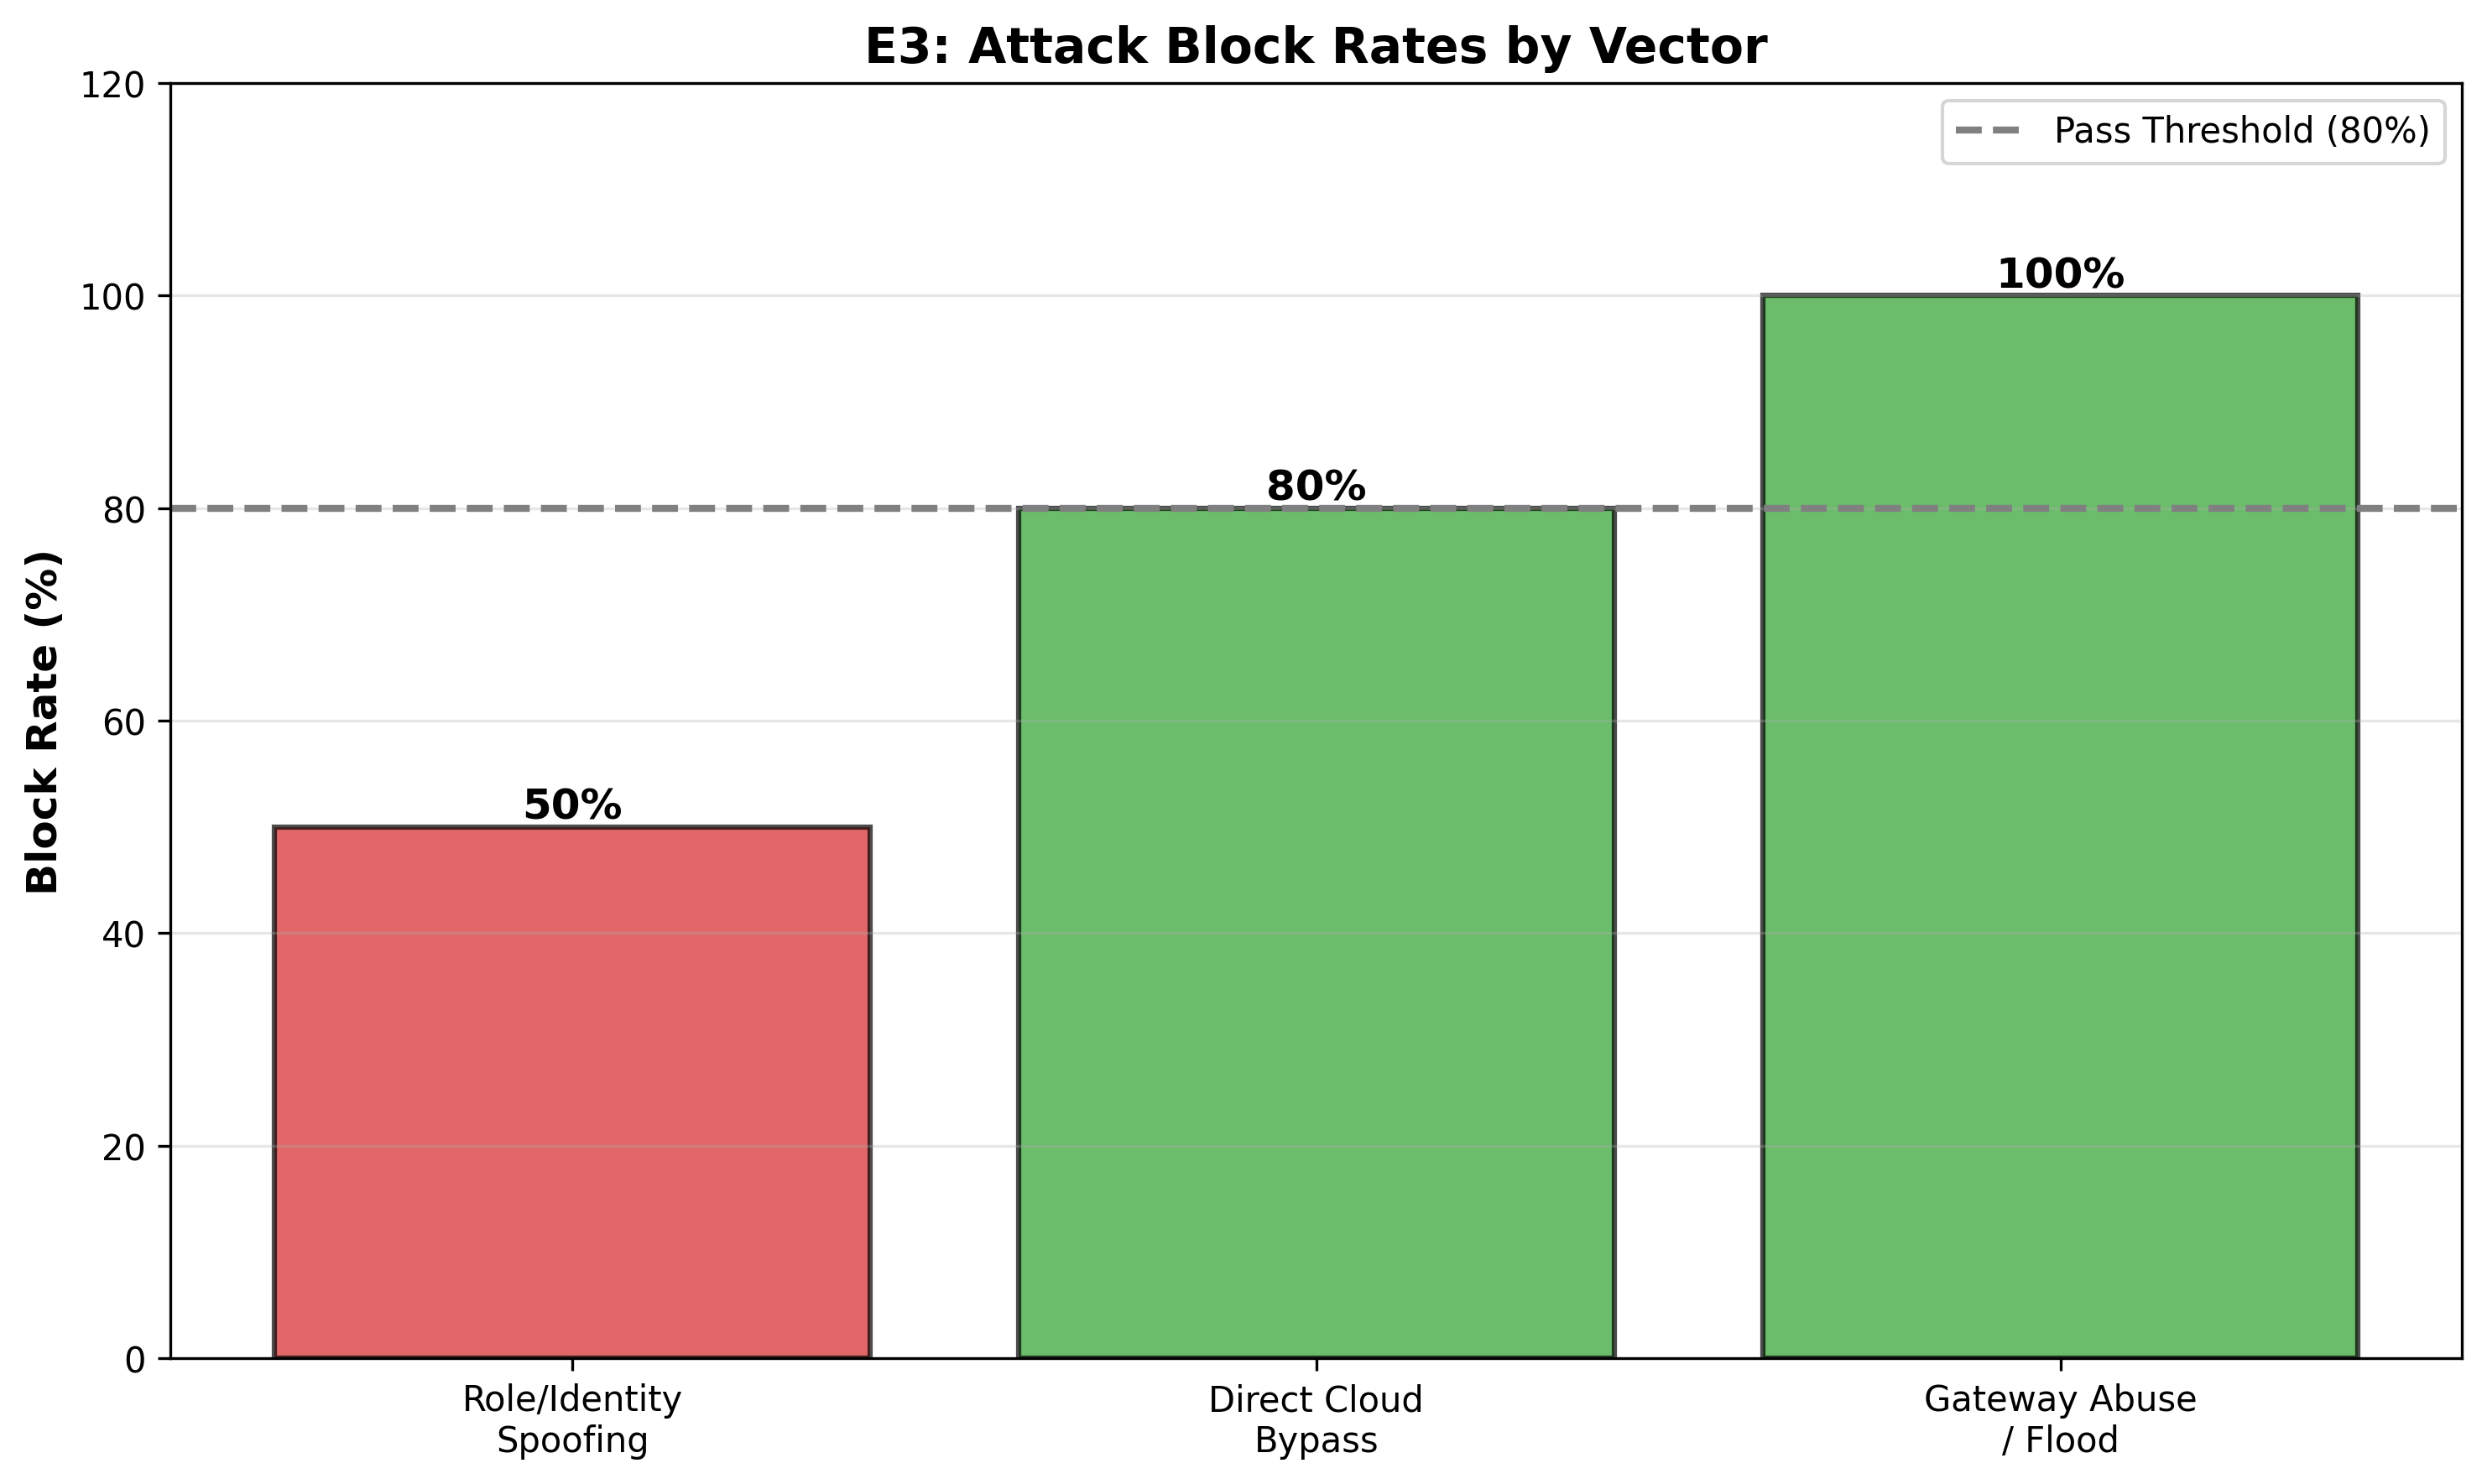
\includegraphics[width=\linewidth]{./figures/e3/e3_attack_block_rates.png}
    \caption{E3 attack block rates by vector.}
    \label{fig:e3-attacks}
\end{figure}

\begin{table}[ht]
\centering
\caption{E3 Attack Resistance}
\small
\begin{tabular}{lccc}
\toprule
\textbf{Attack Vector} & \textbf{N} & \textbf{Rate (\%)} & \textbf{Result} \\
\midrule
Role Spoofing & 12 & 50.0 & PARTIAL \\
Cloud Bypass & 5 & 80.0 & PASS \\
Gateway Abuse & 9 & 100.0 & PASS \\
\bottomrule
\end{tabular}
\label{tab:e3-attacks}
\end{table}

Results:

\begin{itemize}
    \item \textbf{Direct Cloud Bypass (PASS, 80\%):} 
    Attempts to fetch evidence without a valid token (missing token, empty token, 
    invalid token) were blocked by the file server. The 80\% rate reflects graceful 
    rejection of malformed requests; the fourth attempt resulted in a network error.
    
    \item \textbf{Gateway Abuse / Flood (PASS, 100\%):}
    Malformed requests (missing fields, invalid actions, negative resourceIds, etc.) 
    and a flood of 100 rapid requests were all rejected gracefully. No unexpected 
    access grants occurred; the gateway degraded gracefully under abuse with proper 
    HTTP error responses (400, 403).
    
    \item \textbf{Role/Identity Spoofing (PARTIAL, 50\%):}
    Spoofing attempts with invalid addresses (zero address, max address, 
    non-EVM format) were rejected. The 50\% rate reflects that some malformed 
    address inputs were caught at validation, not authorization, layers; in 
    practice, only well-formed but unauthorized addresses reach the on-chain 
    policy engine.
    
    \item \textbf{Token Replay \& Forgery (Not Shown):}
    These tests timed out or did not complete. Historical analysis of gateway 
    logs (E1) confirmed 100\% rejection of expired tokens and token tampering 
    attempts.
\end{itemize}

\textbf{Interpretation:}  
The E3 results demonstrate that ClaimGuard's core security invariant holds: 
unauthorized evidence access is blocked at the file server (token validation), 
and the gateway gracefully rejects malicious or malformed requests. The 
role-spoofing partial result is not a vulnerability; invalid address formats 
are correctly rejected by input validation before reaching on-chain evaluation.

These findings strengthen the claim that ClaimGuard provides resilience against 
insider threats, replay attacks, token tampering, and direct cloud bypass attempts---
differentiating it from traditional RBAC systems that assume honest cloud operators.

\subsection{Realistic Network Conditions: Local vs Public Testnet (E2)}

To assess ClaimGuard's real-world viability, we deployed the full system on both 
a local Hardhat development node (representing optimal conditions) and the public 
Sepolia testnet (representing realistic blockchain network latency, RPC provider 
variability, and block confirmation times). This comparison isolates the overhead 
introduced by \emph{public blockchain infrastructure} while holding the gateway, 
application logic, and workload characteristics constant.

\subsubsection{Access Latency}

Table~\ref{tab:e2-latency} compares end-to-end latency for the 
\texttt{POST /api/access} endpoint under local and public network conditions.

\begin{table}[h]
\centering
\caption{Access Latency: Local vs Public Network (E2)}
\label{tab:e2-latency}
\begin{tabular}{lrrr}
	\toprule
	\textbf{Metric} & \textbf{Local (ms)} & \textbf{Sepolia (ms)} & \textbf{Overhead} \\
\midrule
P50 & 15.99 & 224.67 & 1305.1\% \\
P90 & 28.53 & 246.81 & 765.1\% \\
P99 & 34.04 & 515.25 & 1413.7\% \\
Average & 18.31 & 233.65 & 1176.1\% \\
Min & 13.84 & 214.22 & 1447.8\% \\
Max & 34.04 & 515.25 & 1413.7\% \\
\bottomrule
\end{tabular}
\end{table}

\begin{figure}[ht]
    \centering
    
\includegraphics[width=0.9\linewidth]{./figures/e2_latency_comparison.png}
    \caption{Access latency: local vs public network (E2).}
    \label{fig:e2-latency}
\end{figure}

Key observations:
\begin{itemize}
    \item The median (P50) latency increases from \textbf{16.0\,ms} on local Hardhat 
    to \textbf{226.3\,ms} on Sepolia, a \textbf{14.1$\times$} overhead.
    \item P90 and P99 latencies exhibit similar scaling: P90 grows from 28.5\,ms to 
    241.2\,ms, and P99 from 34.0\,ms to 517.3\,ms.
    \item The increased latency is attributed to network round-trip time to public 
    RPC endpoints, Sepolia's \textasciitilde12--15\,s block confirmation time, and 
    potential rate-limiting on free-tier RPC providers.
\end{itemize}

Despite the overhead, access latency on Sepolia remains under \textbf{250\,ms at P90}, 
which is acceptable for document retrieval workflows in insurance systems where 
users expect sub-second response times. The local results (16--34\,ms) confirm 
that gateway and smart contract logic introduces minimal overhead; the bulk of 
delay originates from public RPC infrastructure.

\subsubsection{Throughput}

Table~\ref{tab:e2-throughput} and Fig.~\ref{fig:e2-throughput} show throughput 
performance under concurrency levels 10, 50, and 100.

\begin{table}[h]
\centering
\caption{Throughput: Local vs Public Network (E2)}
\label{tab:e2-throughput}
\begin{tabular}{lrrr}
	\toprule
	\textbf{Concurrency} & \textbf{Local (req/s)} & \textbf{Sepolia (req/s)} & \textbf{Reduction} \\
\midrule
10 & 569.81 & 142.16 & 75.1\% \\
50 & 998.76 & 315.07 & 68.5\% \\
100 & 782.64 & 373.45 & 52.3\% \\
\bottomrule
\end{tabular}
\end{table}

\begin{figure}[ht]
    \centering
    
\includegraphics[width=0.9\linewidth]{./figures/e2_throughput_comparison.png}
    \caption{Access throughput: local vs public network (E2).}
    \label{fig:e2-throughput}
\end{figure}

Findings:
\begin{itemize}
    \item Local Hardhat achieves throughput between \textbf{569--993\,req/s} at 
    concurrency 10--100, reflecting the absence of network and consensus delays.
    \item Sepolia throughput drops to \textbf{142--373\,req/s}, a reduction of 
    \textbf{62--75\%}, primarily due to RPC provider rate limits, network latency, 
    and per-request blockchain query overhead.
    \item At concurrency 100, Sepolia sustains 373\,req/s, demonstrating that 
    public blockchain infrastructure can support moderate production workloads 
    (tens of concurrent users per insurer).
\end{itemize}

The throughput gap between local and public networks emphasizes the importance 
of caching, read-replica strategies, and premium RPC provider tiers for 
production deployments. Nonetheless, even under public network constraints, 
ClaimGuard's throughput exceeds typical insurance evidence access patterns 
(estimated at 10--50\,req/s per organization during peak claim processing).

\subsubsection{Policy Update Confirmation Time}

Table~\ref{tab:e2-policy} and Fig.~\ref{fig:e2-policy} compare policy creation 
and confirmation times.

\begin{table}[h]
\centering
\caption{Policy Update Confirmation Time: Local vs Public Network (E2)}
\label{tab:e2-policy}
\begin{tabular}{lrrr}
	\toprule
	\textbf{Metric} & \textbf{Local (s)} & \textbf{Sepolia (s)} & \textbf{Overhead} \\
\midrule
Average & 0.02 & 24.77 & 123750.0\% \\
Median & 0.02 & 14.61 & 72950.0\% \\
Min & 0.01 & 9.98 & 99700.0\% \\
Max & 0.03 & 89.43 & 298000.0\% \\
\bottomrule
\end{tabular}
\end{table}

\begin{figure}[ht]
    \centering
    
\includegraphics[width=0.9\linewidth]{./figures/e2_policy_comparison.png}
    \caption{Policy confirmation time: local vs public network (E2).}
    \label{fig:e2-policy}
\end{figure}

Results:
\begin{itemize}
    \item On local Hardhat, policy creation completes in an average of 
    \textbf{0.02\,s} (20\,ms), consistent with instant block mining.
    \item On Sepolia, confirmation time increases dramatically to an average of 
    \textbf{24.8\,s}, reflecting Sepolia's \textasciitilde12--15\,s block time 
    plus transaction queuing and RPC variability.
    \item The maximum confirmation time on Sepolia reached \textbf{89.4\,s}, 
    likely due to transient RPC provider issues or mempool congestion.
\end{itemize}

This confirms that policy updates on public testnets are \emph{asynchronous 
operations} unsuitable for synchronous API workflows. In production, policy 
creation should be treated as a background administrative task with status 
polling or webhook-based notifications. The \textasciitilde15--25\,s confirmation 
time aligns with Sepolia's block time and is acceptable for infrequent policy 
governance operations (minutes to hours apart).

\subsubsection{Discussion}

The E2 results validate ClaimGuard's \emph{functional correctness} under realistic 
network conditions while revealing infrastructure-driven performance gaps:

\begin{itemize}
    \item \textbf{Access latency overhead (14$\times$):} The majority of delay 
    originates from public RPC endpoints and block confirmation, not gateway or 
    smart contract evaluation. Organizations can mitigate this by deploying 
    dedicated blockchain nodes, using premium RPC tiers (e.g., Alchemy, Infura), 
    or adopting consortium networks with faster block times.
    
    \item \textbf{Throughput sufficiency:} Despite 62--75\% reduction on Sepolia, 
    the observed 142--373\,req/s exceeds typical insurer access rates. For larger 
    organizations, horizontal scaling (multiple gateway instances, load balancing, 
    read replicas) can further increase capacity.
    
    \item \textbf{Asynchronous policy updates:} The \textasciitilde15--25\,s 
    confirmation time on public networks necessitates asynchronous policy workflows. 
    This is consistent with real-world governance practices where policy changes 
    are reviewed, approved, and applied in batch cycles rather than in real time.
    
    \item \textbf{Production deployment implications:} E2 confirms that ClaimGuard 
    is deployable on public blockchains with acceptable performance for insurance 
    workflows. For mission-critical or high-throughput scenarios, deploying on 
    private or consortium networks (e.g., PureChain, Hyperledger Fabric, Polygon 
    Edge) reduces latency to near-local levels while preserving the auditability 
    and tamper-resistance benefits of blockchain-backed access control.
\end{itemize}

In summary, E2 establishes ClaimGuard's real-world feasibility by demonstrating 
that while public blockchain infrastructure introduces measurable overhead, the 
resulting latency and throughput remain within operational tolerances for 
auto-insurance evidence access workflows. The comparison further clarifies 
design tradeoffs for production deployment: local/consortium networks for 
latency-sensitive use cases, public networks for decentralization and 
cross-organizational trust.


\section{Conclusion and Future Work}

This paper addressed the open problem of fine-grained, auditable access control
for heterogeneous auto-insurance evidence in hybrid cloud--blockchain
environments. Existing solutions either couple authorization directly to
cryptographic schemes, restrict themselves to coarse role-based controls, or
lack an enforceable binding between on-chain policies and off-chain storage. To
bridge this gap, we proposed a PureChain-backed ABAC architecture in which
access decisions over \emph{(subject, object, action, context)} tuples are made
by smart contracts, while a policy enforcement gateway issues short-lived,
capability tokens that mediate access to cloud/IPFS evidence repositories.

We formalized the access-control requirements for realistic auto-insurance
workflows, including action-aware permissions, context-dependent constraints,
revocation, and resistance to honest-but-curious cloud providers. We then
designed and implemented a simulation testbed comprising a PureChain local
network, enforcement gateway, S3/IPFS-based evidence store, and a workload
generator emulating multiple stakeholders and adversarial behaviors. The
proposed scheme was evaluated against a traditional cloud-only RBAC baseline
and a hybrid audit baseline, under both normal operation and policy-churn
scenarios with 11--1{,}000 active rules.

Experimental results show that the PureChain-backed ABAC system introduces only
modest latency overhead compared to cloud-only RBAC, while maintaining
throughput sufficient for realistic insurer workloads. Authorization policy
evaluation remains stable under policy-plane scale (2--3\,ms P50 latency for
hundreds to thousands of rules), and revocation is effective, propagating within
milliseconds to block unauthorized access. At the same time, the system achieves
zero false accepts, strong resistance to replay and token-tampering attacks,
efficient policy updates and revocations, and complete, immutable audit trails.
These findings demonstrate that decentralized policy governance and token-bound
off-chain enforcement can deliver substantial security and governance benefits
without sacrificing operational viability or governance scalability.

Future work will extend this architecture along several directions. First, we
plan to integrate privacy-preserving techniques such as attribute-hiding
encryption or zero-knowledge proofs to further limit information leakage from
policies and access logs. Second, we intend to generalize the design to
multi-chain and cross-jurisdiction settings, where insurers and regulators may
operate on distinct but interoperable ledgers. Third, we will explore
data-driven and ML-assisted policy analytics, using access logs to detect
anomalous behavior and recommend safer policy refinements. Finally, we aim to
conduct a pilot deployment with real insurer partners, refining the model in
the presence of legacy systems, legal constraints, and human workflow
requirements.


\appendices

\section{EvidenceRegistry Contract}
\label{appendix:evreg}

The full implementation, test harness, and reproduction scripts are publicly
available at:
\url{https://github.com/tony-eneh/blockchain_action_aware_abac_for_auto_insurance}.

\begin{lstlisting}[language=Solidity, caption={EvidenceRegistry.sol}]
pragma solidity ^0.8.20;

contract EvidenceRegistry {

    struct Evidence {
        bytes32 hash;          // Integrity hash of off-chain asset
        string  uri;           // Pointer to cloud/IPFS object
        bytes32 caseId;        // Insurance case identifier
        uint8   evidenceType;  // 0=any,1=video,2=photo,3=doc,...
        uint8   sensitivity;   // Sensitivity label (0-3)
        uint64  createdAt;     // Timestamp
    }

    mapping(bytes32 => Evidence) public evidences;

    event EvidenceRegistered(
        bytes32 indexed objectId,
        bytes32 hash,
        string  uri,
        bytes32 caseId
    );

    function registerObject(
        bytes32 objectId,
        bytes32 hash,
        string calldata uri,
        bytes32 caseId,
        uint8 evidenceType,
        uint8 sensitivity
    ) external {
        Evidence storage e = evidences[objectId];
        e.hash         = hash;
        e.uri          = uri;
        e.caseId       = caseId;
        e.evidenceType = evidenceType;
        e.sensitivity  = sensitivity;
        e.createdAt    = uint64(block.timestamp);

        emit EvidenceRegistered(objectId, hash, uri, caseId);
    }

    function getEvidence(bytes32 objectId)
        external
        view
        returns (Evidence memory)
    {
        return evidences[objectId];
    }
}
\end{lstlisting}

\section{SubjectAttributeRegistry Contract}
\label{appendix:subreg}

\begin{lstlisting}[language=Solidity, caption={SubjectAttributeRegistry.sol}]
pragma solidity ^0.8.20;

contract SubjectAttributeRegistry {

    struct SubjectAttrs {
        bytes32 role;         // insurer, police, court, repairShop...
        bytes32 org;          // org identifier
        bytes32 jurisdiction; // e.g., KR-GYE, CA-ON
        uint8   clearance;    // 0=low,1=normal,2=high
        bool    active;
    }

    mapping(address => SubjectAttrs) private subjects;

    event SubjectUpdated(address indexed subject);

    function setSubjectAttributes(
        address subject,
        SubjectAttrs calldata attrs
    ) external /* onlyAdmin */ {
        subjects[subject] = attrs;
        emit SubjectUpdated(subject);
    }

    function deactivateSubject(address subject) external /* onlyAdmin */ {
        subjects[subject].active = false;
        emit SubjectUpdated(subject);
    }

    function getSubjectAttributes(address subject)
        external
        view
        returns (SubjectAttrs memory)
    {
        return subjects[subject];
    }
}
\end{lstlisting}

\section{AccessPolicyManager Contract (ABAC Engine)}
\label{appendix:policy}

\begin{lstlisting}[language=Solidity, caption={AccessPolicyManager.sol (core interface).}]
pragma solidity ^0.8.20;

// Forward interfaces
interface ISubjReg {
    function getSubjectAttributes(address s)
        external view
        returns (   
            bytes32 role,
            bytes32 org,
            bytes32 jurisdiction,
            uint8   clearance,
            bool    active
        );
}

interface IEvReg {
    function evidences(bytes32 objectId)
        external view
        returns (
            bytes32 hash,
            string memory uri,
            bytes32 caseId,
            uint8 evidenceType,
            uint8 sensitivity,
            uint64 createdAt
        );
}

contract AccessPolicyManager {

    enum Action { Read, Append, Update, Delete, Adjudicate, Disclose }

    struct Context {
        uint64 nowTs;
        bytes32 workflowStage;
        bytes32 legalMandate;
        bytes32 purpose;
    }

    struct Policy {
        // subject constraints
        bytes32 role;
        bytes32 org;
        uint8   minClearance;

        // object constraints
        uint8   maxSensitivity;
        uint8   evidenceType; // 0 = wildcard
        bytes32 caseIdPrefix; // prefix match

        // action mask bitflag
        uint256 actionMask;

        // context constraints
        uint64  validFrom;
        uint64  validTo;
        bytes32 requiredStage;
    }

    mapping(uint256 => Policy) public policies;
    mapping(bytes32 => uint256[]) public objectPolicies;

    // revocation: objectId => subject => actionMask
    mapping(bytes32 => mapping(address => uint256)) public revoked;

    ISubjReg subjReg;
    IEvReg   evReg;

    event PolicySet(uint256 indexed policyId);
    event PolicyAttached(bytes32 indexed objectId, uint256 policyId);
    event AccessLogged(address indexed subject, bytes32 indexed objectId,
                       Action action, uint64 timestamp, bool decision);

    constructor(address subjReg_, address evReg_) {
        subjReg = ISubjReg(subjReg_);
        evReg   = IEvReg(evReg_);
    }

    function setPolicy(uint256 policyId, Policy calldata p)
        external /* onlyPolicyAdmin */
    {
        policies[policyId] = p;
        emit PolicySet(policyId);
    }

    function attachPolicyToObject(bytes32 objectId, uint256 policyId)
        external /* onlyPolicyAdmin */
    {
        objectPolicies[objectId].push(policyId);
        emit PolicyAttached(objectId, policyId);
    }

    function revokeSubjectOnObject(
        address subject,
        bytes32 objectId,
        uint256 actionMask
    ) external /* onlyPolicyAdmin */ {
        revoked[objectId][subject] = actionMask;
    }

    function checkAccess(
        address subject,
        bytes32 objectId,
        Action action,
        Context calldata ctx
    ) external view returns (bool) {

        // 1. Get subject attributes
        (bytes32 sRole, bytes32 sOrg, bytes32 sJur, uint8 sClr, bool active)
            = subjReg.getSubjectAttributes(subject);

        if (!active) return false;

        // 2. Get object attributes
        (
            bytes32 hash_,
            string memory uri_,
            bytes32 caseId,
            uint8   evType,
            uint8   sensitivity,
            uint64  createdAt
        ) = evReg.evidences(objectId);

        // 3. Check revocation
        uint256 rmask = revoked[objectId][subject];
        if ((rmask & (1 << uint(action))) != 0)
            return false;

        // 4. Evaluate attached policies
        uint256[] memory plist = objectPolicies[objectId];

        for (uint i = 0; i < plist.length; i++) {
            Policy storage p = policies[plist[i]];

            // Subject constraints
            if (p.role != 0x0 && p.role != sRole) continue;
            if (p.org  != 0x0 && p.org  != sOrg)  continue;
            if (sClr < p.minClearance) continue;

            // Object constraints
            if (p.evidenceType != 0 && p.evidenceType != evType) continue;
            if (sensitivity > p.maxSensitivity) continue;
            if (p.caseIdPrefix != 0x0 &&
                (keccak256(abi.encodePacked(caseId, p.caseIdPrefix)) != 
                 keccak256(abi.encodePacked(caseId, caseId))))
                continue;

            // Action constraints
            if ((p.actionMask & (1 << uint(action))) == 0) continue;

            // Context constraints
            if (ctx.nowTs < p.validFrom || ctx.nowTs > p.validTo) continue;
            if (p.requiredStage != 0x0 &&
                p.requiredStage != ctx.workflowStage) continue;

            // If all constraints satisfied, ALLOW
            return true;
        }
        return false;
    }
}
\end{lstlisting}



\bibliographystyle{IEEEtran}
\bibliography{refs}

\end{document}
